\chapter{Análisis colección \#BLM}
\label{chap:blm}
Es importante recordar que el trabajo previo de: la comparación entre algoritmos de perfilado de usuarios y el análisis, diseño e implementación de una herramienta para analizar las publicaciones de usuarios de redes sociales; viene motivado por la necesidad de extraer información acerca del fenómeno social \acrfull{blm}.

Concretamente, en este capítulo se aplicará nuestro sistema para conocer mejor el tipo de usuarios que publicaban en el corpus, en idioma español, construido por \cite{heritage_BLM} en 2020 a modo de archivo social sobre sobre las discusiones acerca de los conflictos raciales motivados por el asesinato de George Floyd. Este corpus se encuentra disponible en \url{https://www.dc.fi.udc.es/~david/hdh2021/}.
\subsection{Procesado corpus}
Al bajar el corpus de la dirección anterior, este viene distribuido entre múltiples archivos XML por cada \textit{thread} o <<hilo>> del subreddit de BLM. Esta agrupación tiene sentido ya que cada <<hilo>> representa un tópico distinto y los comentarios en cada uno tienen un contexto común. Sin embargo, para nuestra finalidad de perfilar cada usuario de la colección tiene mayor importancia usar el mayor número de publicaciones por usuario para que de esta forma las predicciones tengan mayor fiabilidad.
% \begin{verbatim}
% <thread>
%     <id>477</id>
%     <relevant-posts>
%         <id>479</id>
%     </relevant-posts>
%     <posts>
%         <post>
%             <id>479</id>
%             <author>478</author>
%             <body>
%                 >Eso no se de donde lo sacás. Si quieren prohibir el racismo ...
%             </body>
%         </post>
%         ...
%     </posts>
% </thread>

% \end{verbatim}

En este sentido, se procedió a crear un único archivo CSV, con dos columnas: identificador del usuario y texto de la publicación. Este CSV contendrá todas las publicaciones de cada autor de la colección sin tener en cuenta el hilo concreto de cada una. Es importante señalar que no se agrupan las publicaciones de cada autor en una fila, sino que cada publicación de partida se escribe en una fila distinta del csv. De esta forma, al tener las publicaciones de cada autor separadas, cada algoritmo de perfilado se encarga de unirlas y preprocesarlas de la manera oportuna.

\section{Aplicación}
Posteriormente, tras haber creado este archivo CSV con el conjunto de todas las publicaciones de los autores de \acrshort{blm} ya se puede subir a la aplicación para perfilar el corpus. Para ello, arrancamos la aplicación en el entorno local y accedemos desde un navegador a la dirección de \textit{localhost} en el puerto 3000. Tras este paso se podrá ver una página de inicio como la de la figura \ref{fig:app/home}. En cada figura de esta sección se mostrarán dos subfiguras con las vistas de la aplicación desde: ordenador de sobremesa (\textit{desktop}) y móvil (\textit{mobile}).

\begin{figure}[H]
  \centering
  \begin{subfigure}{0.7\textwidth}
       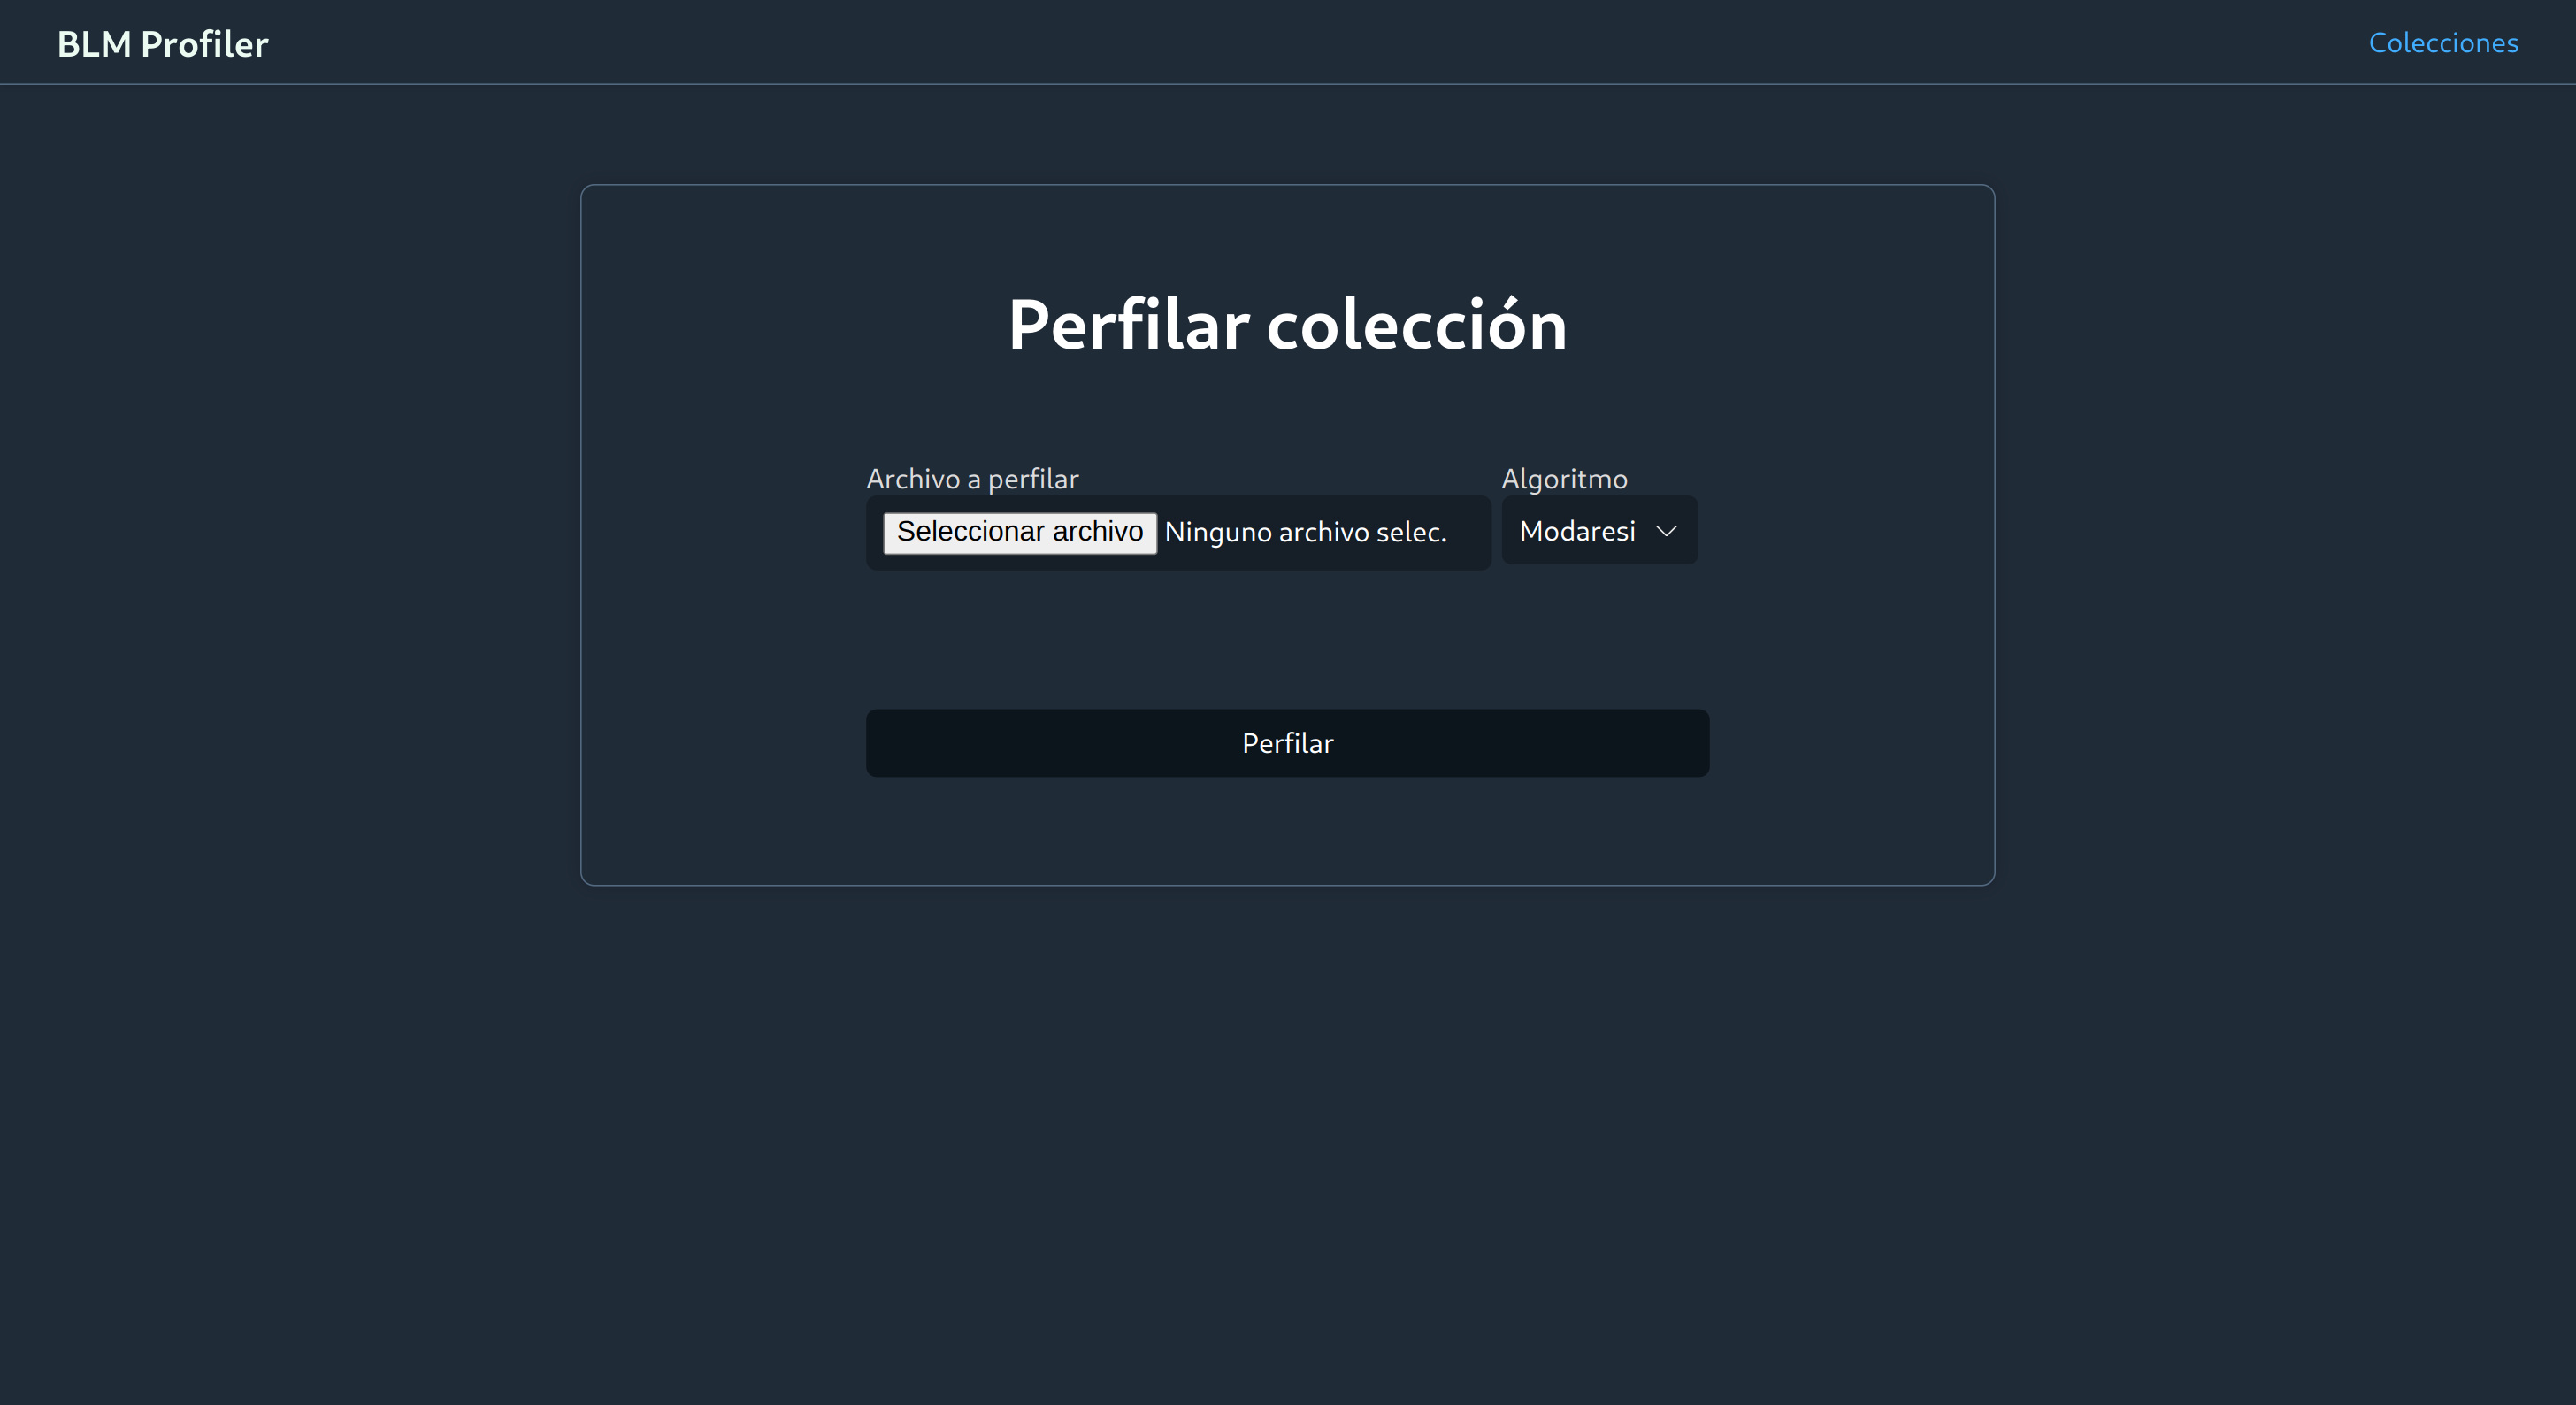
\includegraphics[width=\textwidth]{imaxes/capturas-app/desktop/home.png}
      \caption{\textit{Desktop}} 
  \end{subfigure}
  \begin{subfigure}{0.2215\textwidth}
       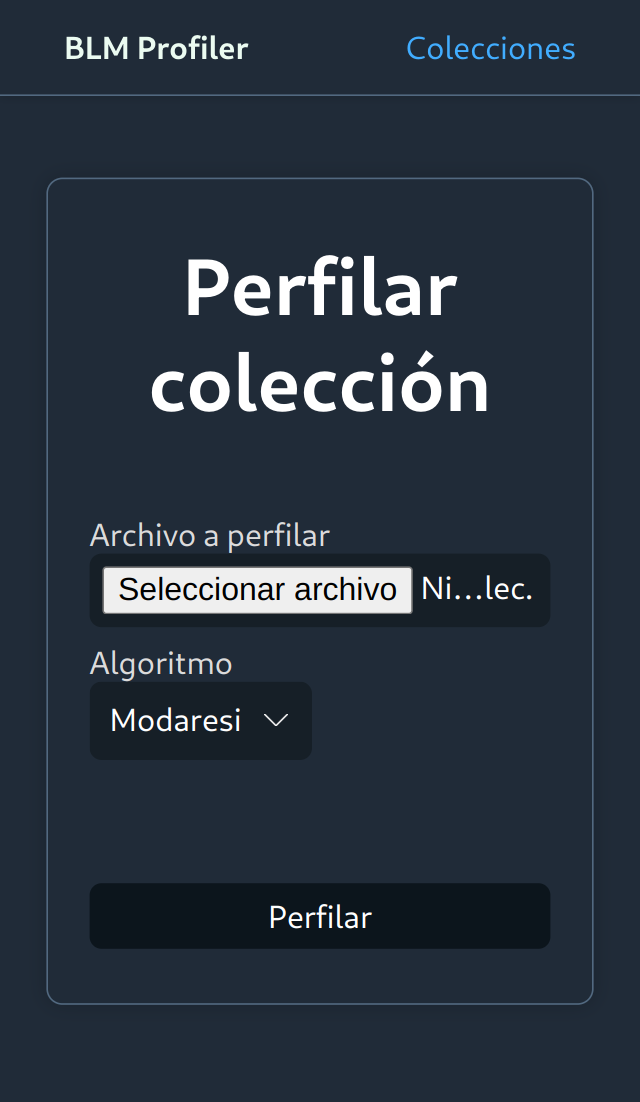
\includegraphics[width=\textwidth]{imaxes/capturas-app/mobile/home.png}
      \caption{\textit{Mobile}} 
  \end{subfigure}
  \caption{Página de inicio.}
  \label{fig:app/home}
\end{figure}
\subsection{Perfilado del corpus}

En esta página se puede ver un formulario con dos campos: uno obligatorio que es el selector del fichero que contiene el corpus a perfilar y otro opcional selector para escoger el algoritmo de perfilado deseado, que por defecto será el de <<modaresi>>. Tras seleccionar el fichero que contiene el corpus a perfilar, que debe tener extensión .csv o .txt, se nos mostrará un mensaje en función de si este es válido o no para el perfilado\footnote{Para que el fichero sea válido debe tener al menos dos columnas llamadas \textit{id} y \textit{posts}, que se refieren al identificador del usuario y su publicación.}. En función de ello nos dejará o no perfilar la colección. Tras este paso si podremos pulsar el botón de perfilar y la página mostrará un spinner a modo de carga mientras se perfila la colección como se puede ver en la figura \ref{fig:app/home-perfilando}.

\begin{figure}[H]
  \centering
  \begin{subfigure}{0.7\textwidth}
       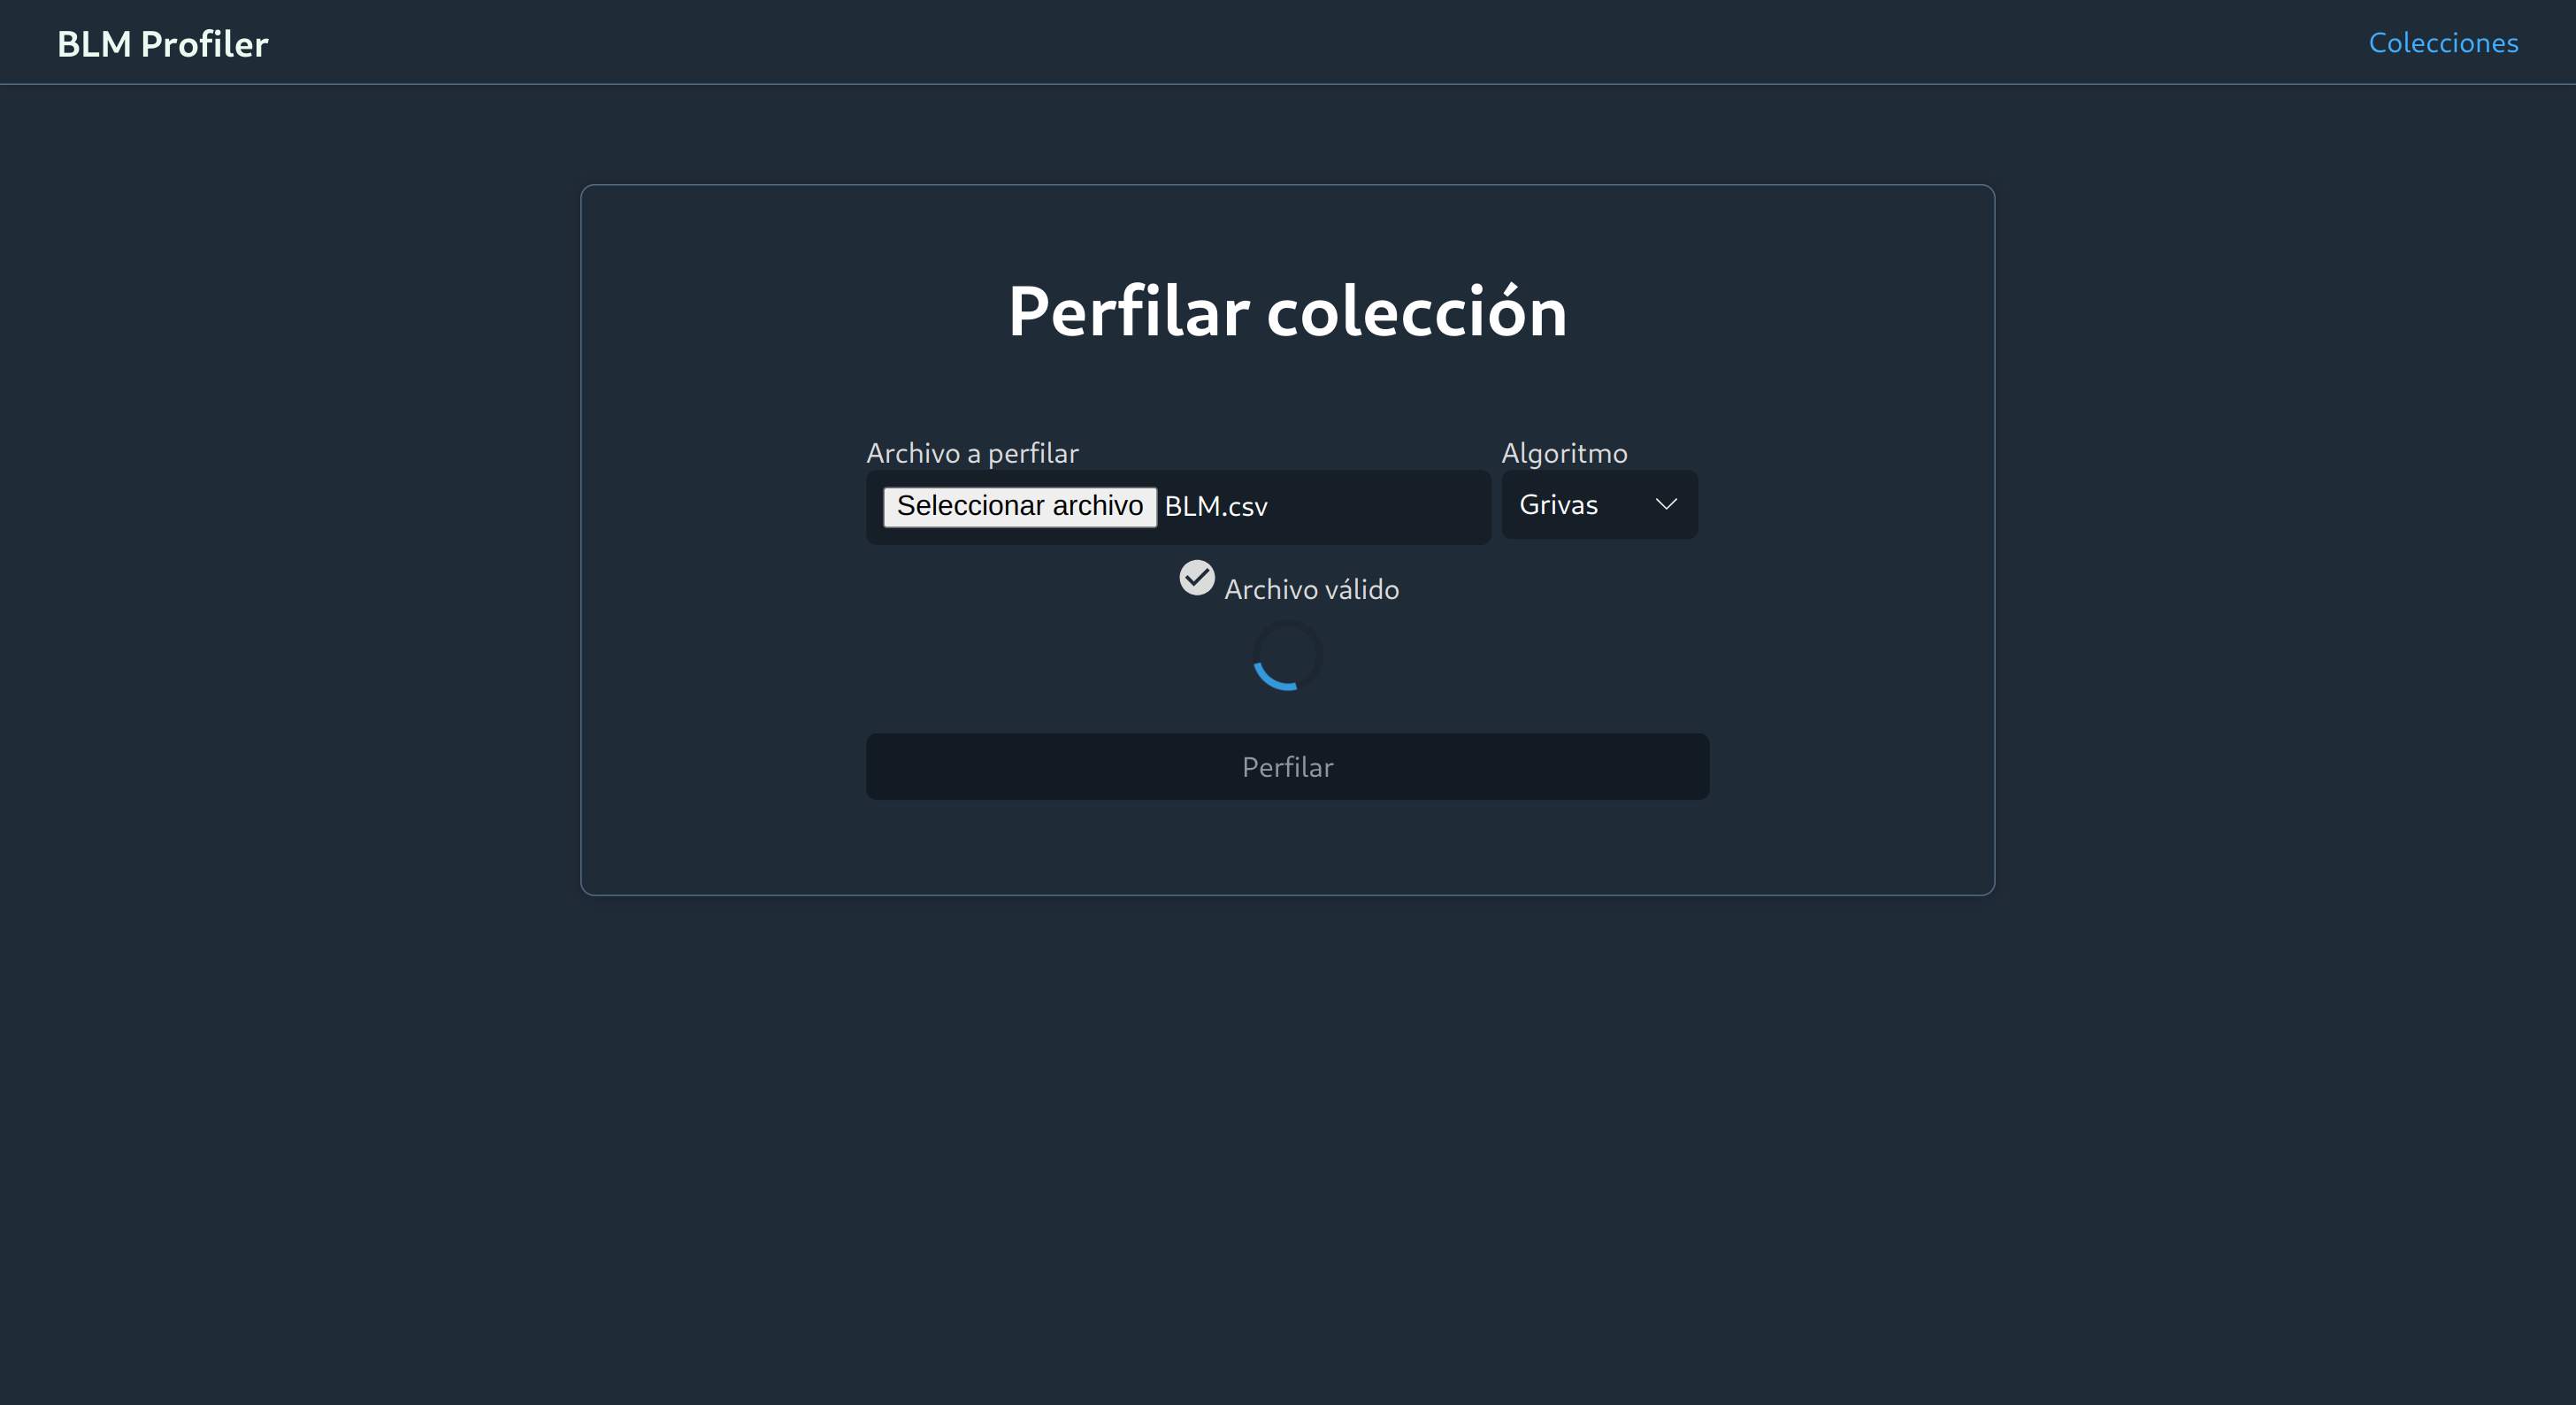
\includegraphics[width=\textwidth]{imaxes/capturas-app/desktop/home_perfilando.png}
      \caption{Desktop} 
  \end{subfigure}
  \begin{subfigure}{0.2215\textwidth}
       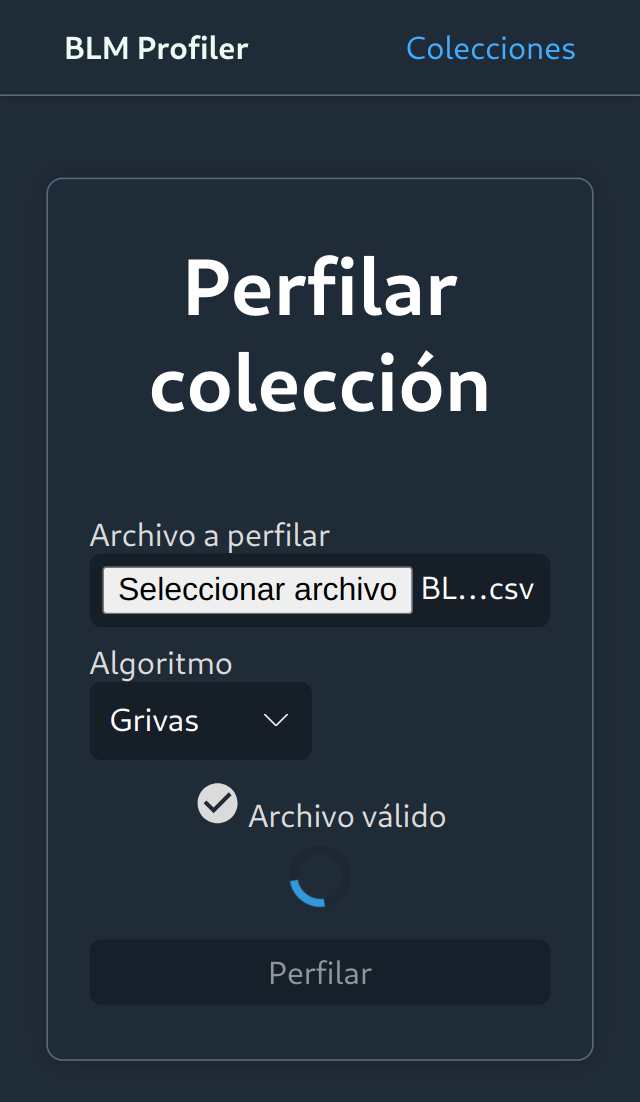
\includegraphics[width=\textwidth]{imaxes/capturas-app/mobile/home_perfilando.png}
      \caption{Mobile} 
  \end{subfigure}
  \caption{Página de inicio mientras se perfila una colección.}
  \label{fig:app/home-perfilando}
\end{figure}
\subsection{Visualización de resultados}

Cuando termine el perfilado la aplicación nos redirigirá al \textit{dashboard} o cuadro de mando de la misma que se puede ver en la figura \ref{fig:app/dashboard}.

\begin{figure}[H]
  \centering
  \begin{subfigure}{0.7\textwidth}
   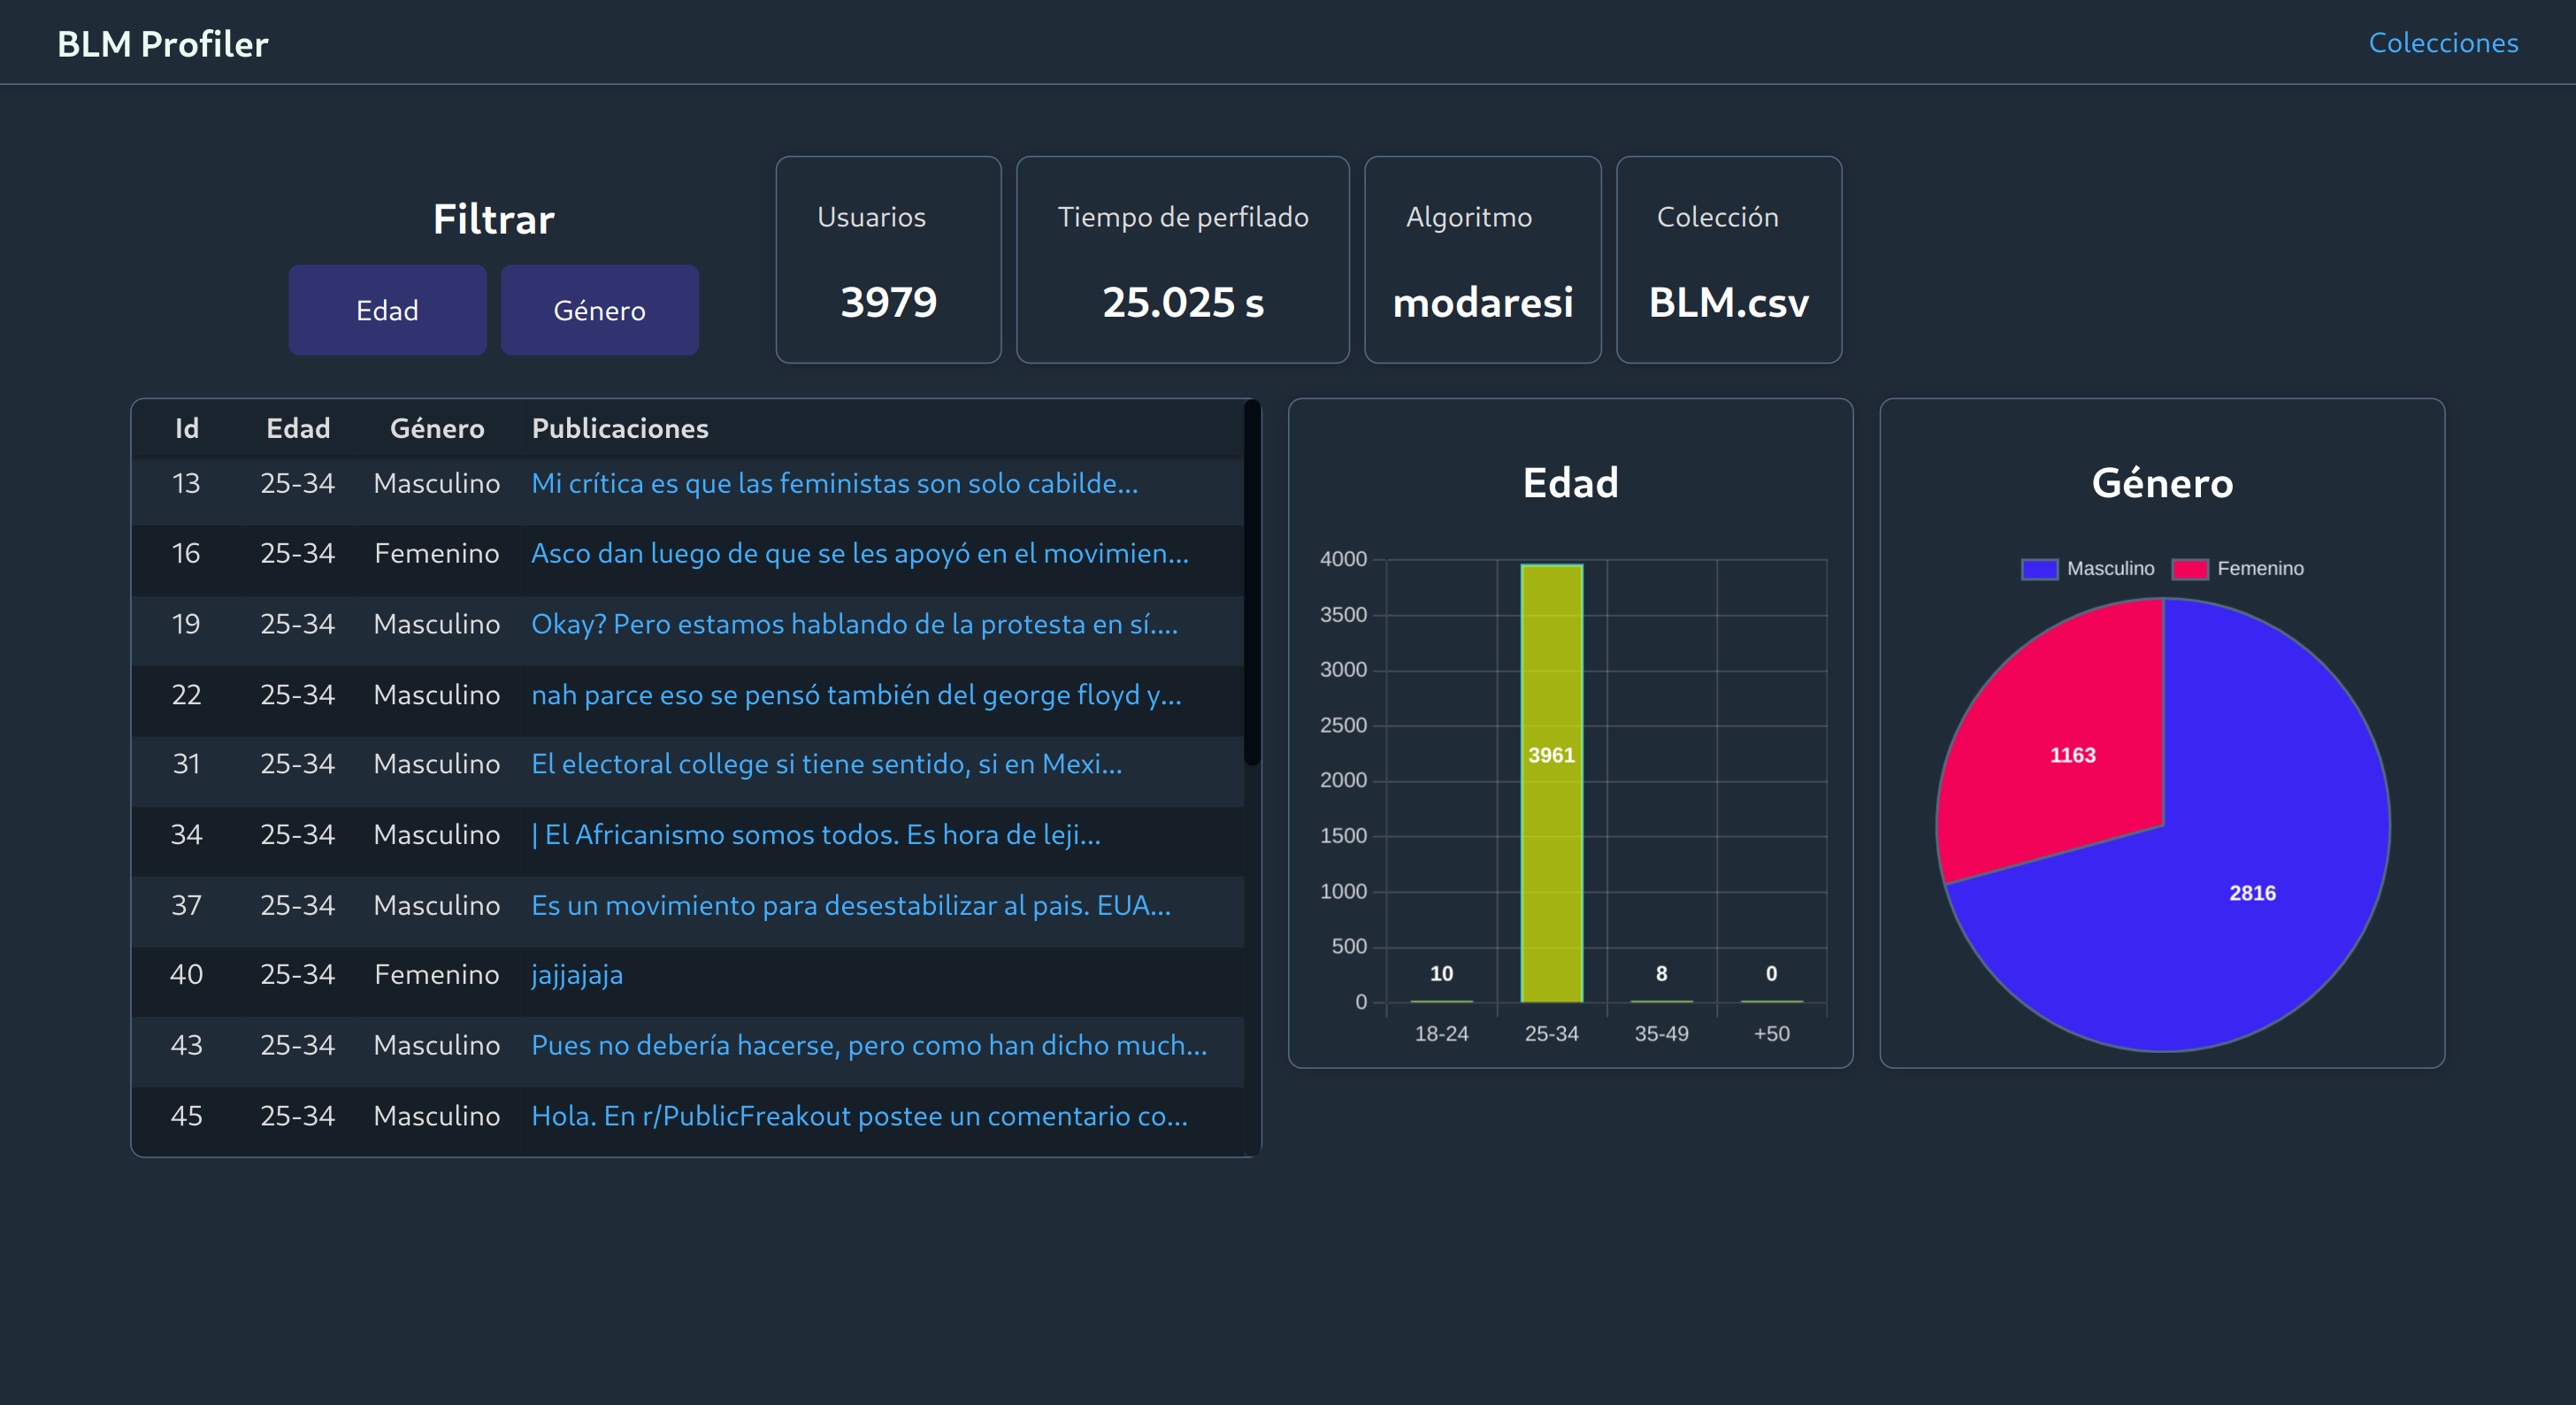
\includegraphics[width=\textwidth]{imaxes/capturas-app/desktop/dashboard.png}
  \caption{\textit{Desktop}} 
  \end{subfigure}
  \begin{subfigure}{0.2215\textwidth}
   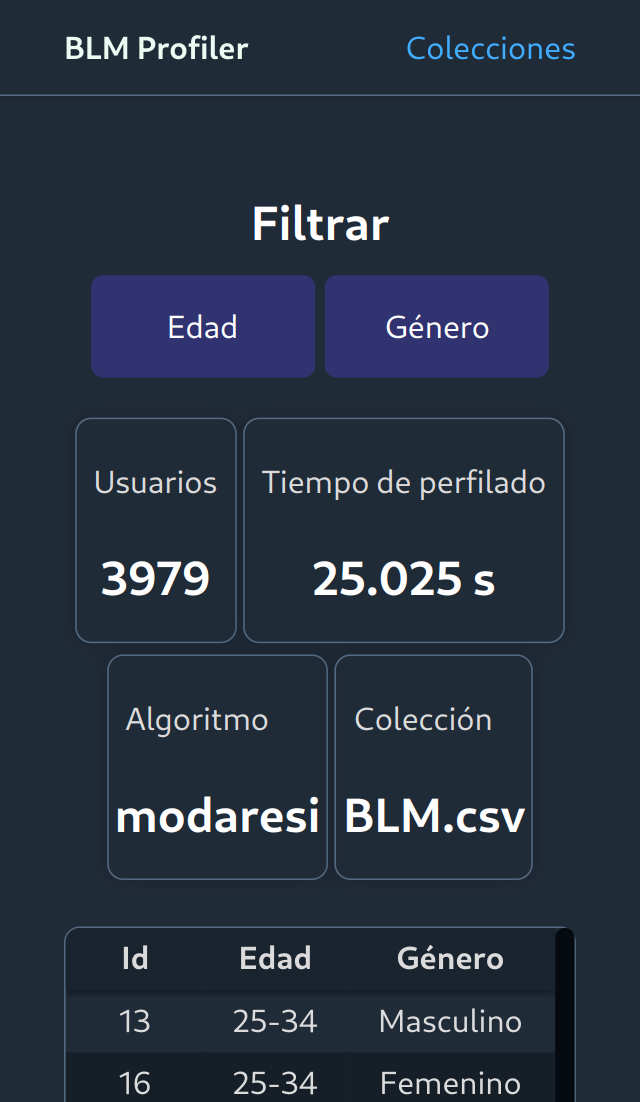
\includegraphics[width=\textwidth]{imaxes/capturas-app/mobile/dashboard.png}
  \caption{\textit{Mobile}} 
  \end{subfigure}
  \caption{\textit{Dashboard} de la colección perfilada.}
  \label{fig:app/dashboard}
\end{figure}

Como podemos ver en la parte de abajo tenemos una tabla y dos gráficos. En el gráfico de barras se puede ver la distribución de los usuarios del corpus según su edad, hay cuatro barras para cuatro rangos de edad distintos. En el gráfico en forma de tarta, en cambio, se muestra la distribución de los usuarios en función del género de los mismos. La tabla, por otra parte, es un listado de todos los usuarios del corpus en el que se muestra el id del mismo\footnote{Correspondiente a la columna id del archivo de subida de la colección}, el género y edad con los que fue clasificado y una muestra de una publicación del usuario en forma de enlace, que explicaremos más adelante.

Luego, en la parte superior, se encuentran varias tarjetas que presentan detalles generales sobre la colección, tales como el tiempo de perfilado, el algoritmo utilizado, el nombre del archivo de subida y el número total de usuarios.

\subsubsection{Filtrado de usuarios por categorías}
Por último, al inicio de la página se encuentra un texto titulado <<Filtrar>> y debajo podemos ver dos botones. Al situar el ratón sobre cualquiera de ellos veremos como realmente son botones desplegables en los que se presentan los posibles filtros para cada categoría. Al seleccionar un filtro de alguna de las categorías veremos como se añade un elemento después de las tarjetas de la colección, que indica el filtro concreto escogido para esa categoría. En la figura \ref{fig:app/dashboard-filtered}, podemos ver el aspecto del filtro añadido.

\begin{figure}[H]
  \centering
  \begin{subfigure}{0.7\textwidth}
   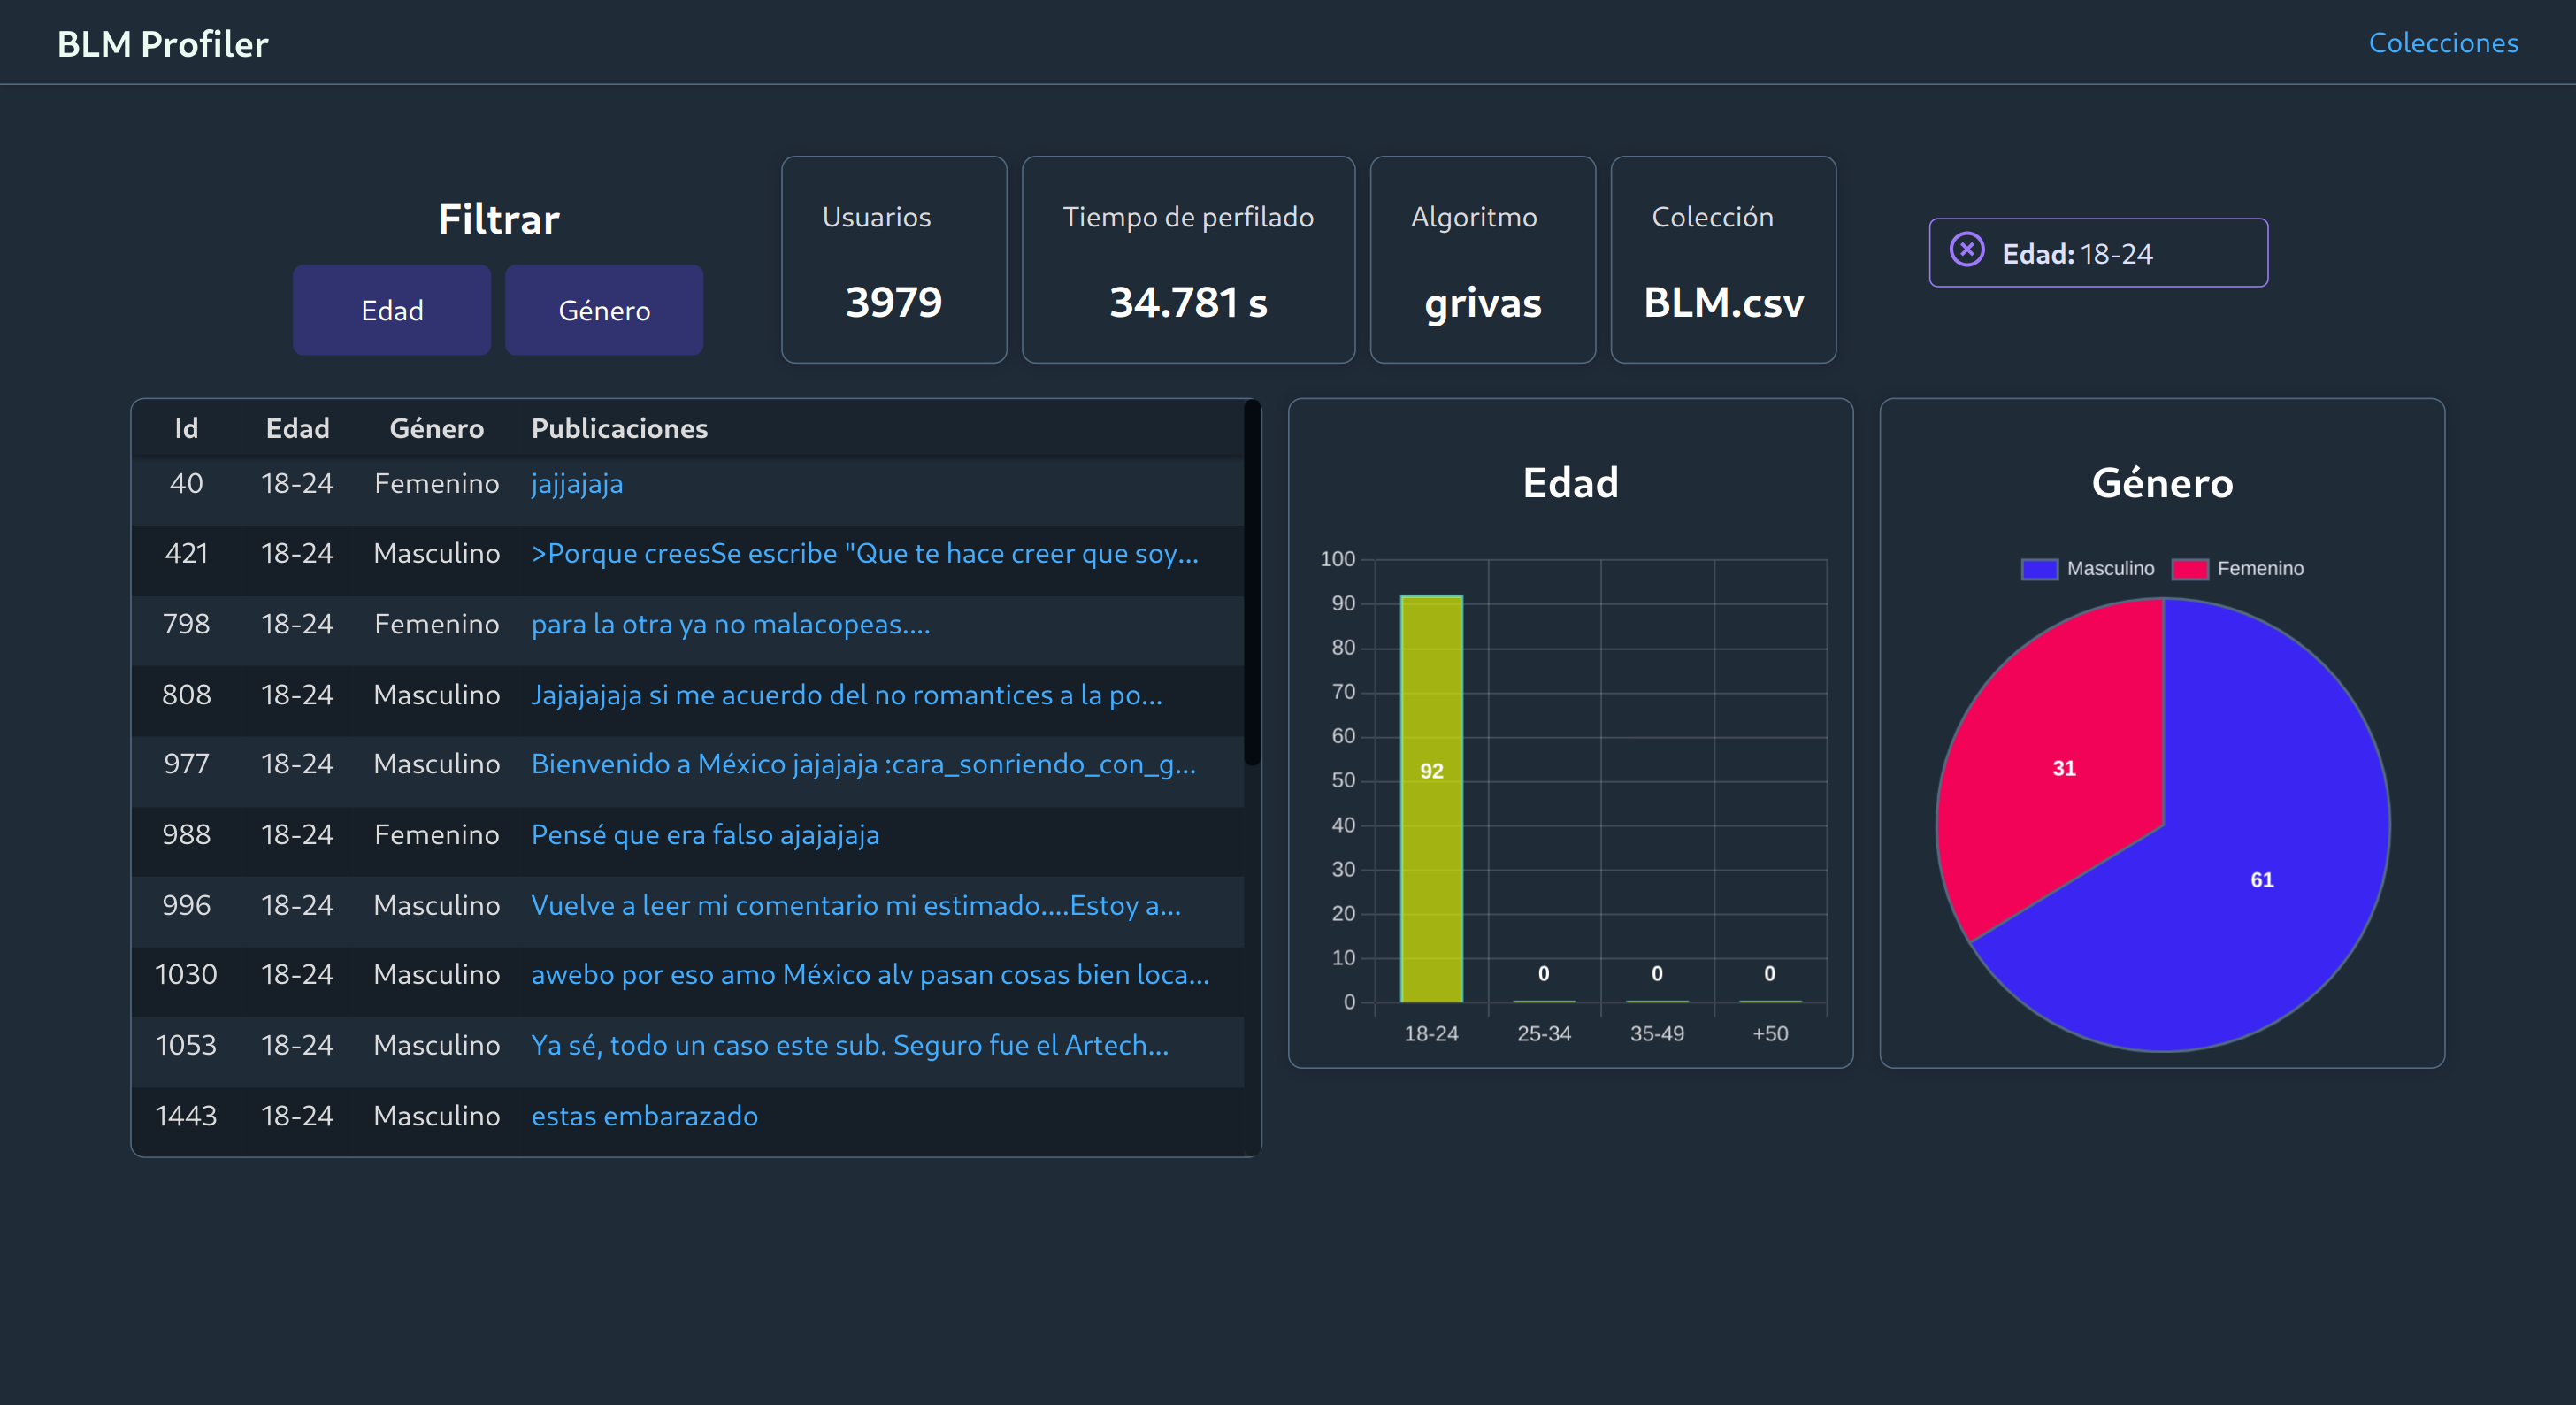
\includegraphics[width=\textwidth]{imaxes/capturas-app/desktop/dashboard-perfilado-edad.png}
  \caption{\textit{Desktop}} 
  \end{subfigure}
  \begin{subfigure}{0.223\textwidth}
   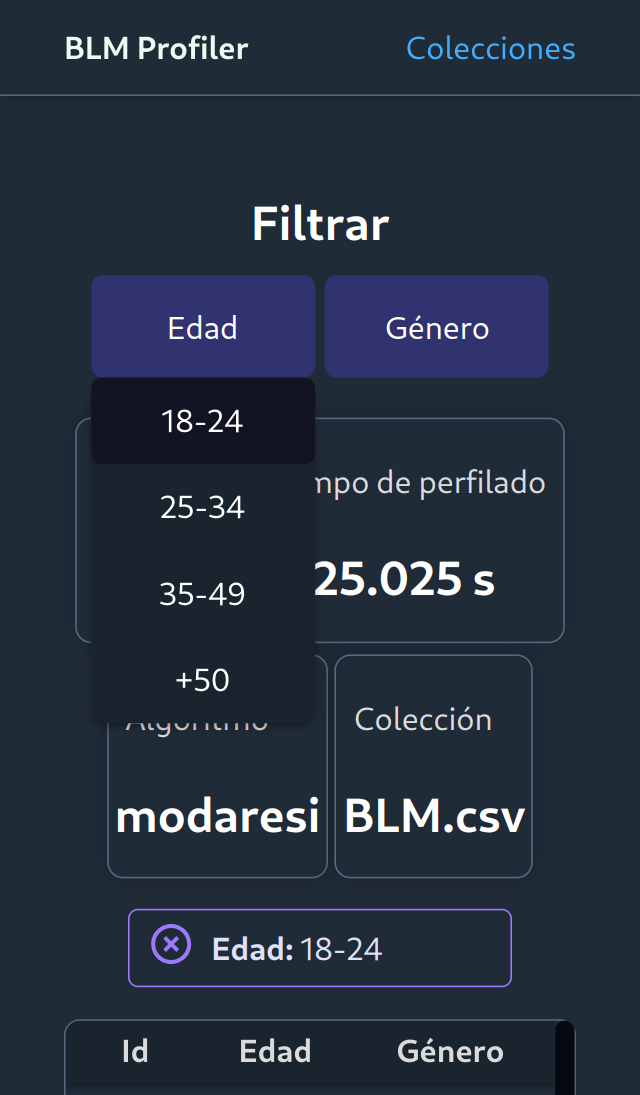
\includegraphics[width=\textwidth]{imaxes/capturas-app/mobile/dashboard-filtrado-edad.png}
  \caption{\textit{Mobile}} 
  \end{subfigure}
  \caption{\textit{Dashboard} de la colección perfilada filtrado únicamente por edad.}
  \label{fig:app/dashboard-filtered}
\end{figure}

Como se puede apreciar en este caso, el proceso de filtrado afecta a la lista de usuarios y a ambos gráficos. Por un lado, en la lista, podemos observar que únicamente se muestran usuarios cuyas edades se sitúan en el rango de 18-24 años. En el gráfico de edad, el filtrado por una grupo de la misma categoría no es especialmente interesante, ya que no nos aporta información nueva. Sin embargo, en el gráfico de género el filtrado por edad nos permite estudiar como cambia la distribución del género de los usuarios en función del rango de edad de los mismos.

Otra opción relevante, es la de filtrar el \textit{dashboard} por ambas categorías. Como ya hemos comentado en los gráficos nos brindaría ninguna información nueva. Por el contrario, al realizar este filtrado podemos estudiar el tipo de publicaciones que realiza un grupo demográfico concreto lo que también nos aporta pistas sobre los criterios que se emplean en el perfilado de cada grupo. En la figura \ref{fig:app/dashboard-filtered-edad-genero}, se puede contemplar el filtrado en función de ambas categorías.

\begin{figure}[H]
  \centering
  \begin{subfigure}{0.7\textwidth}
   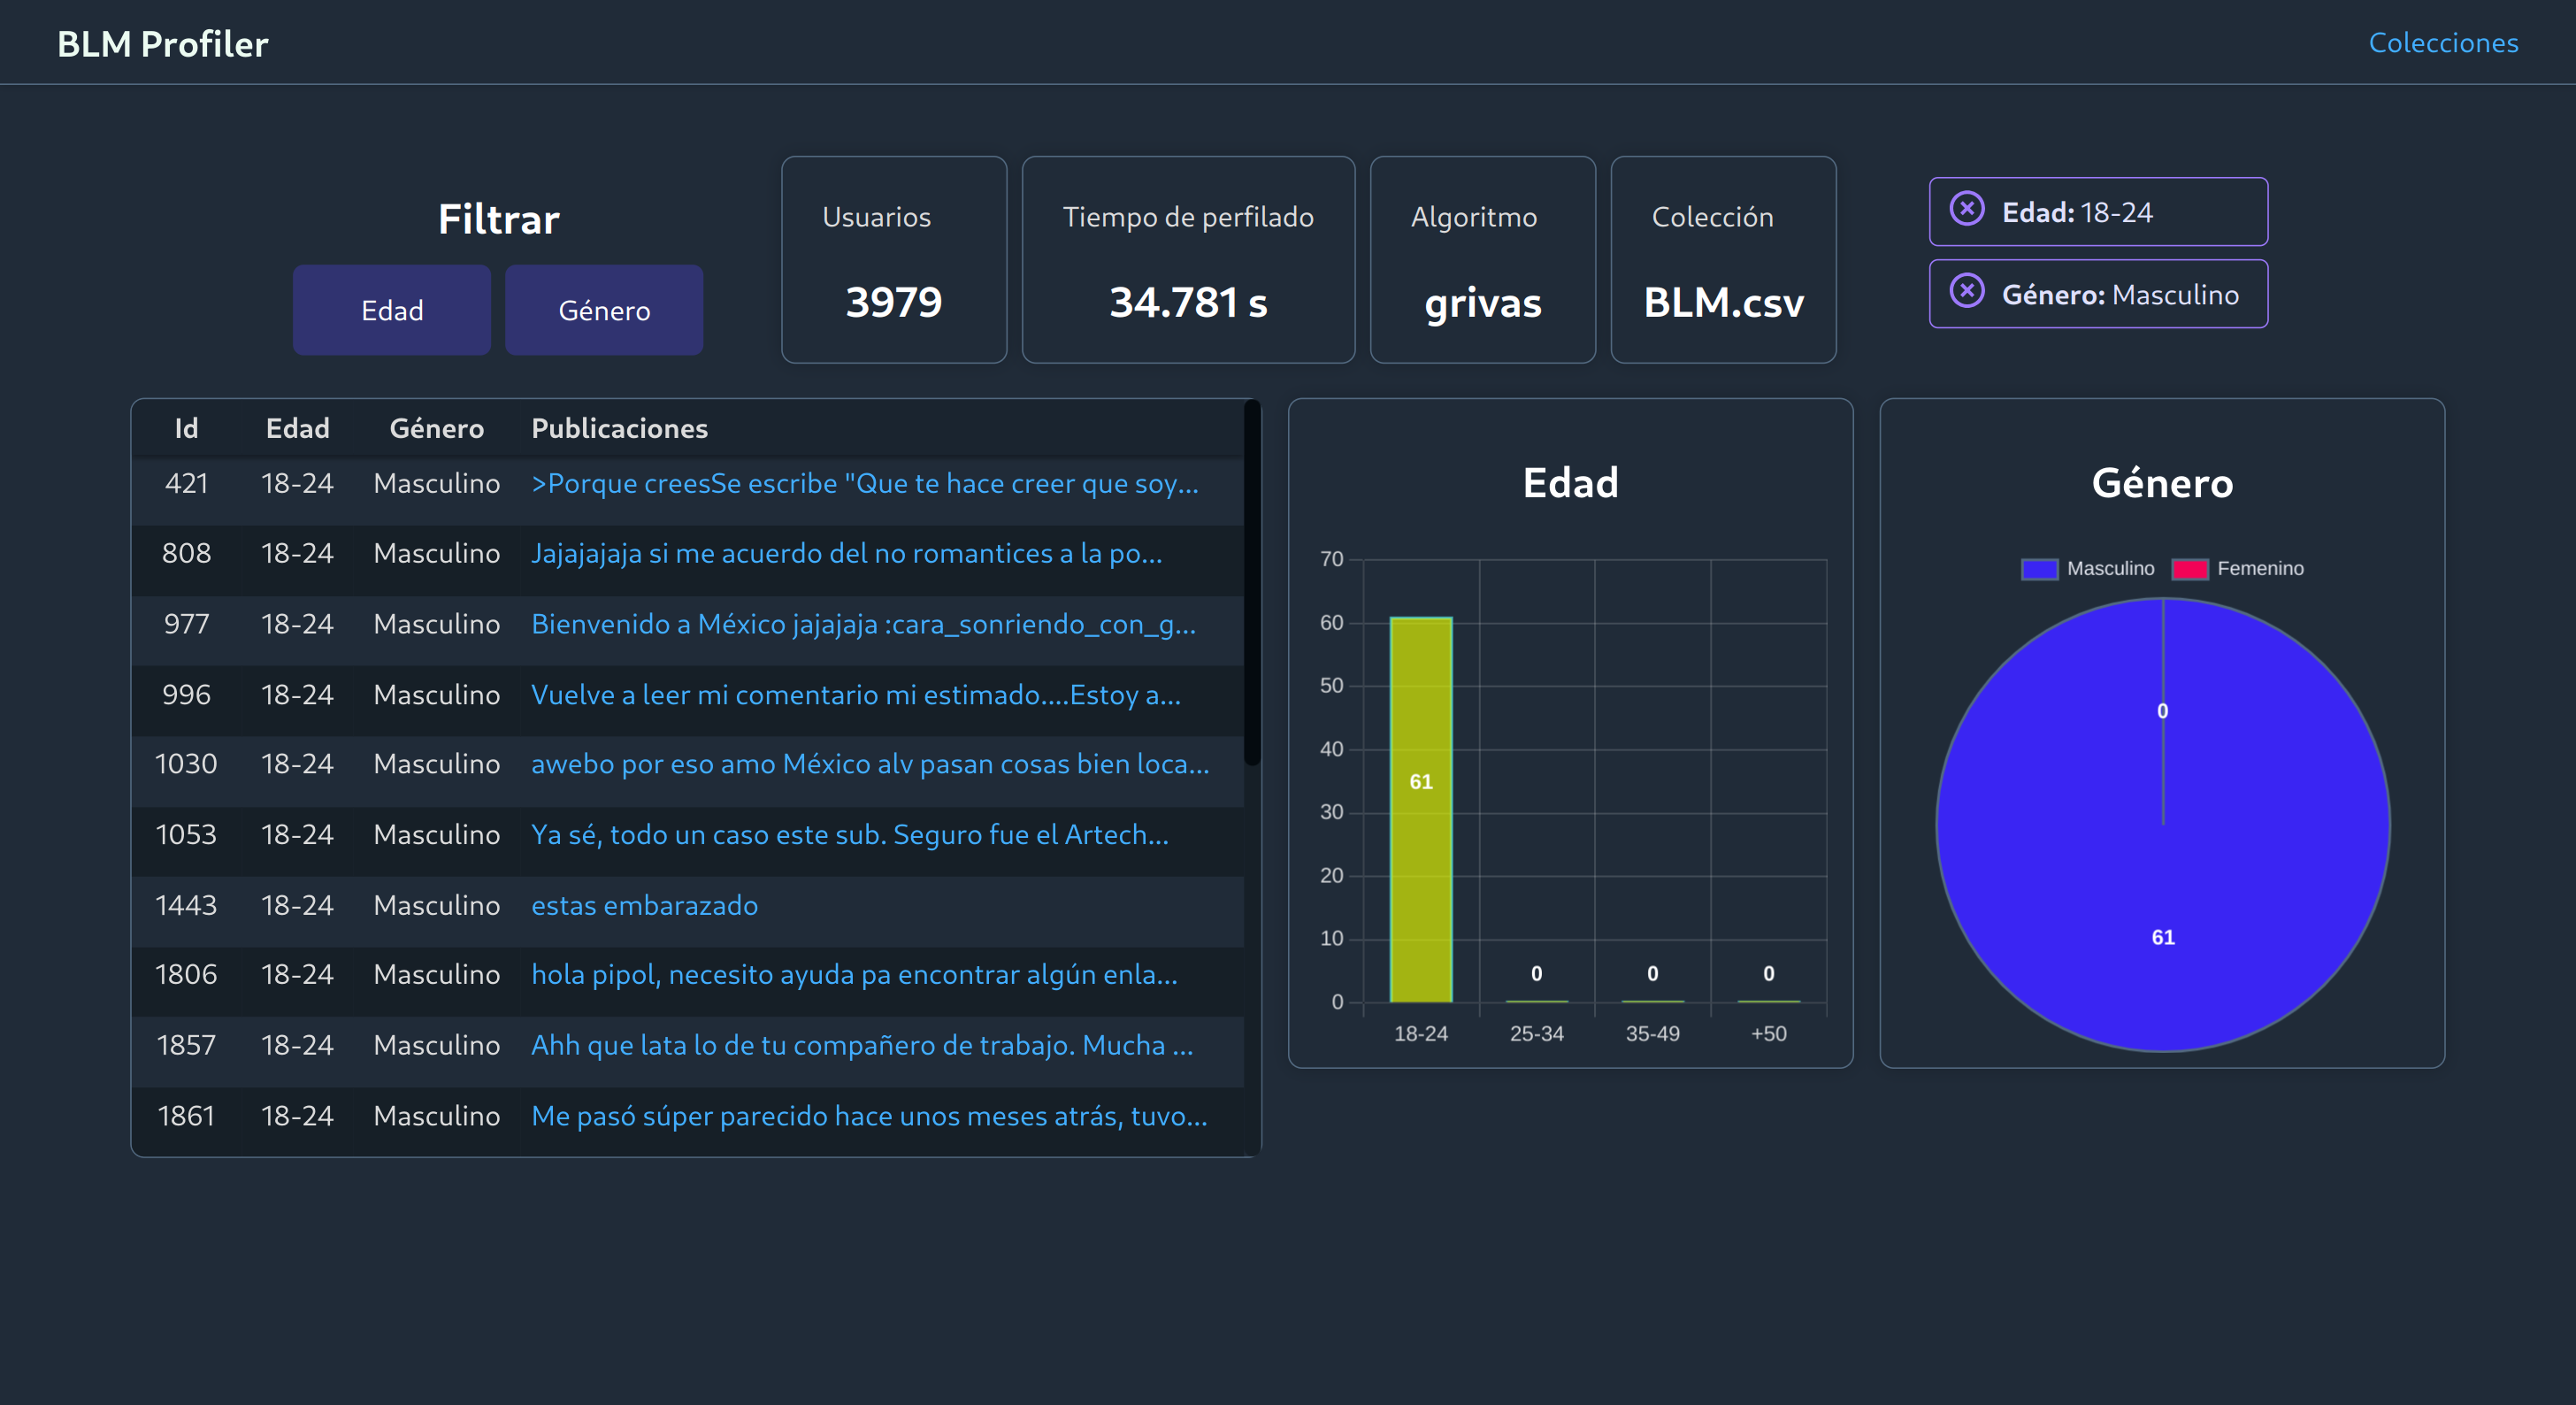
\includegraphics[width=\textwidth]{imaxes/capturas-app/desktop/dashboard-perfilado-edad-genero.png}
  \caption{\textit{Desktop}} 
  \end{subfigure}
  \begin{subfigure}{0.223\textwidth}
   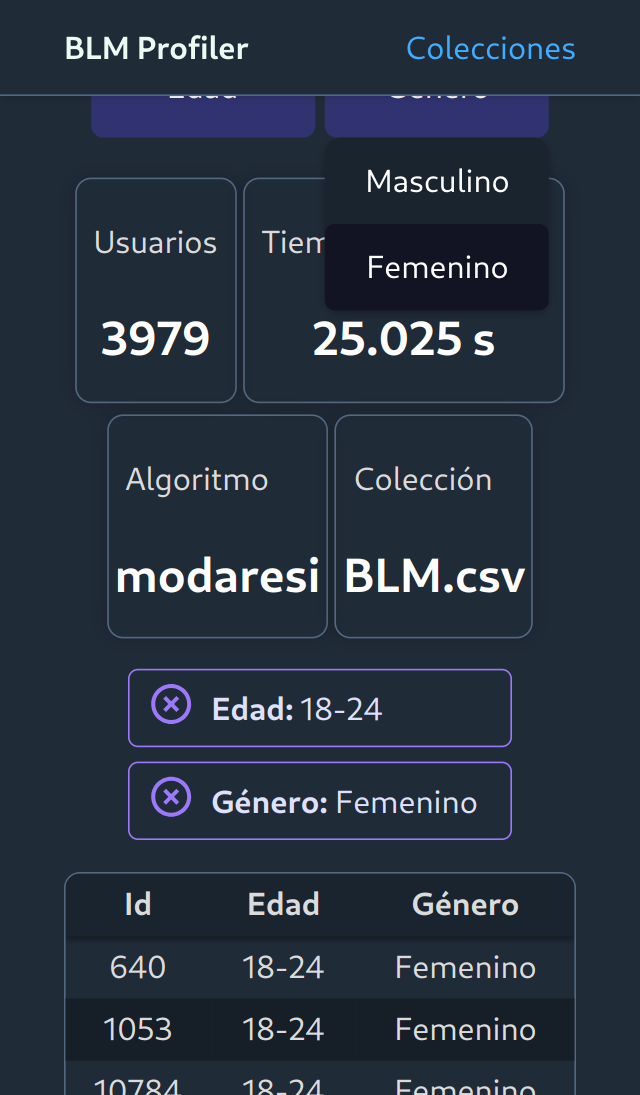
\includegraphics[width=\textwidth]{imaxes/capturas-app/mobile/dashboard-filtrado-edad-genero.png}
  \caption{\textit{Mobile}} 
  \end{subfigure}
  \caption{\textit{Dashboard} de la colección perfilada filtrado por género y edad.}
  \label{fig:app/dashboard-filtered-edad-genero}
\end{figure}

\subsection{Publicaciones de un usuario}
Por ejemplo, si deseáramos examinar el modo en que una usuaria que se encuentra en el rango de edades de 18 a 24 años redacta, tendríamos dos opciones. En la versión de escritorio, podríamos hacer clic en el enlace ubicado en la columna "Publicaciones". Mientras que en la versión móvil, podríamos lograrlo simplemente seleccionando una fila de la tabla. Al realizar esta acción, accederíamos a las publicaciones de la usuaria seleccionada en una página similar a la que se muestra en la figura de referencia.
Por ejemplo, si deseáramos examinar el estilo de redacción de un usuario masculino de entre 25 a 34 años, haríamos clic sobre el enlace de la columna <<Publicaciones>> en la versión \textit{desktop}, o directamente seleccionando una fila de la tabla, en la versión \textit{mobile}. Con esta acción podríamos ver las publicaciones del usuario seleccionado en una página similar a la de la figura \ref{fig:app/user-info}.

\begin{figure}[H]
  \centering
  \begin{subfigure}{0.7\textwidth}
   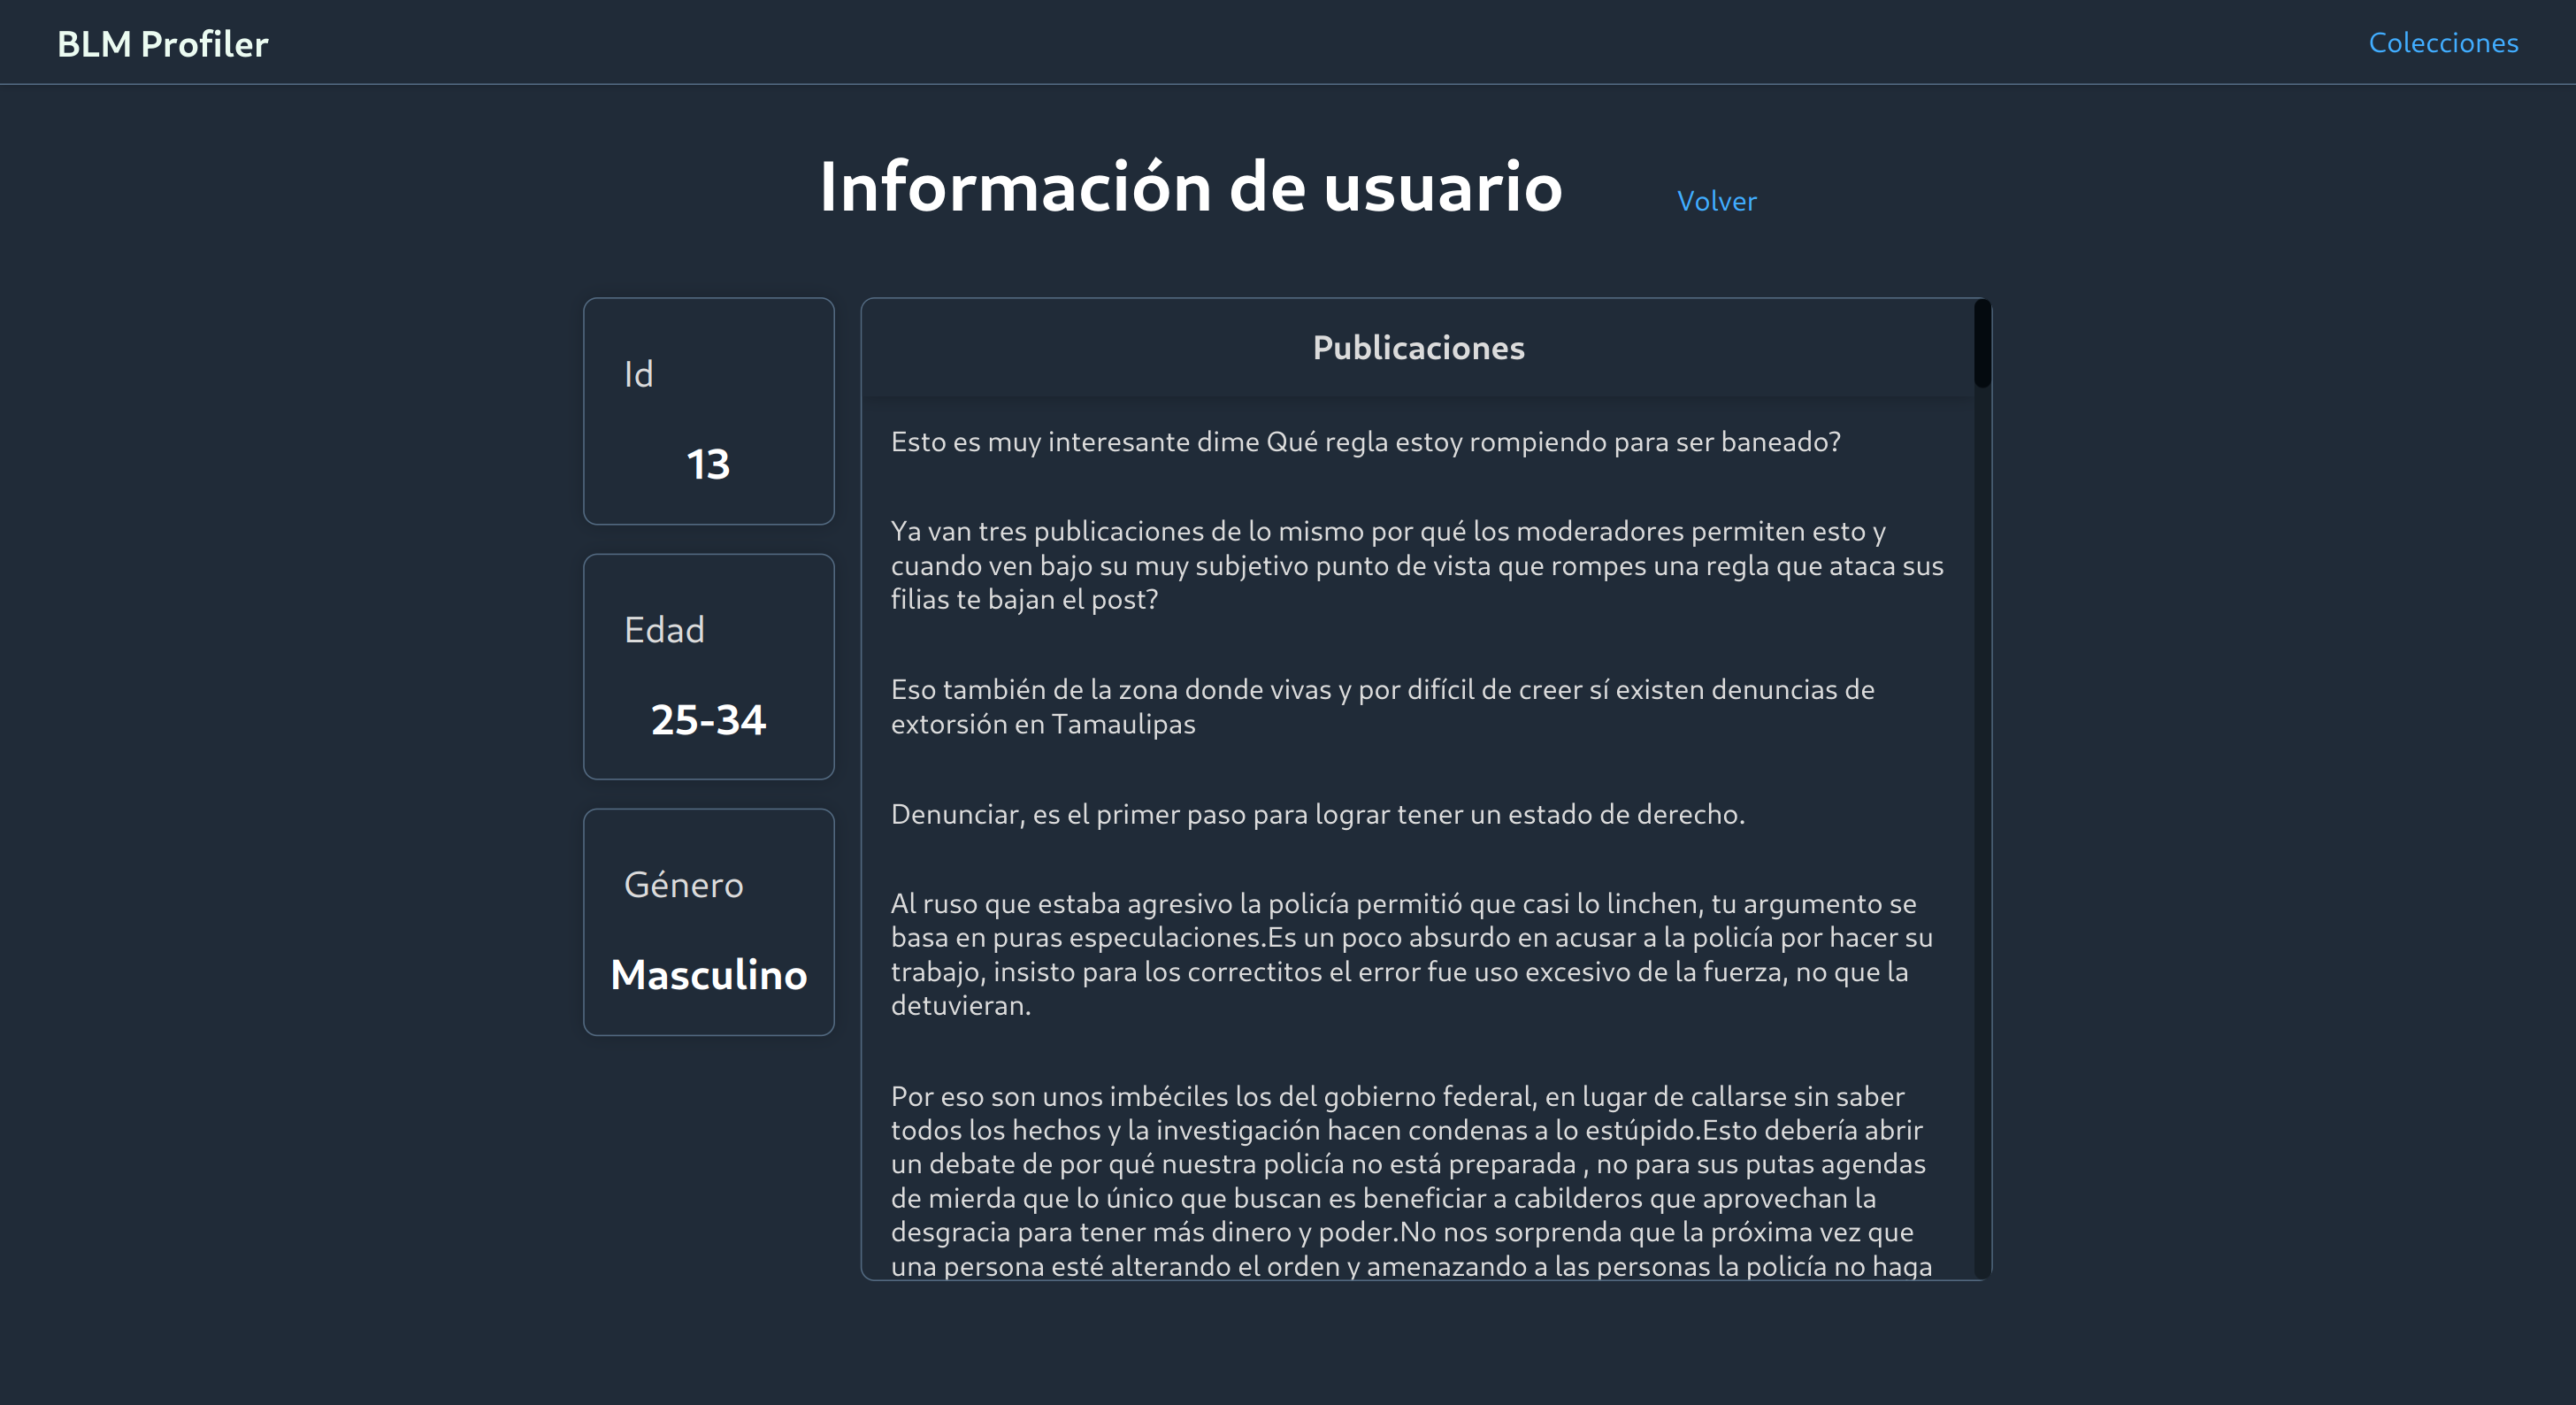
\includegraphics[width=\textwidth]{imaxes/capturas-app/desktop/info-usuario.png}
  \caption{\textit{Desktop}} 
  \end{subfigure}
  \begin{subfigure}{0.223\textwidth}
   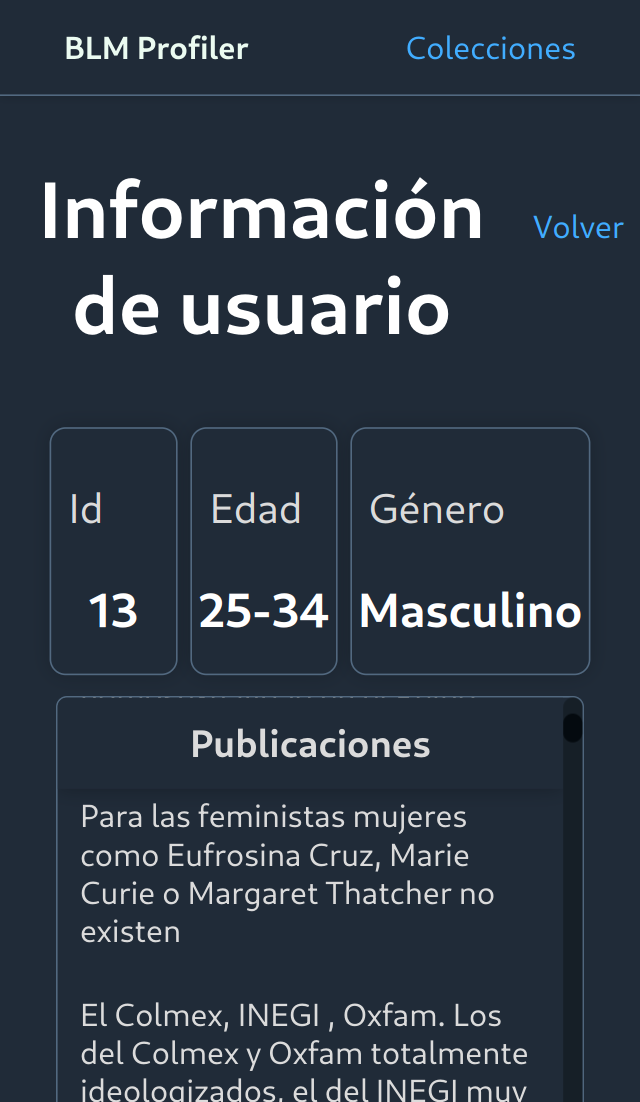
\includegraphics[width=\textwidth]{imaxes/capturas-app/mobile/info-usuario.png}
  \caption{\textit{Mobile}} 
  \end{subfigure}
  \caption{Página de la vista en detalle de un usuario de la colección.}
  \label{fig:app/user-info}
\end{figure}

\subsection{Listado de colecciones}
En cambio, si no deseamos perfilar una colección nueva sino que queremos ver el listado histórico de colecciones ya perfiladas, en la barra de navegación tenemos un enlace, arriba a la derecha, llamado <<Colecciones>> que nos llevará a una página como la de la figura \ref{fig:app/colecciones}. 

\begin{figure}[H]
  \centering
  \begin{subfigure}{0.7\textwidth}
   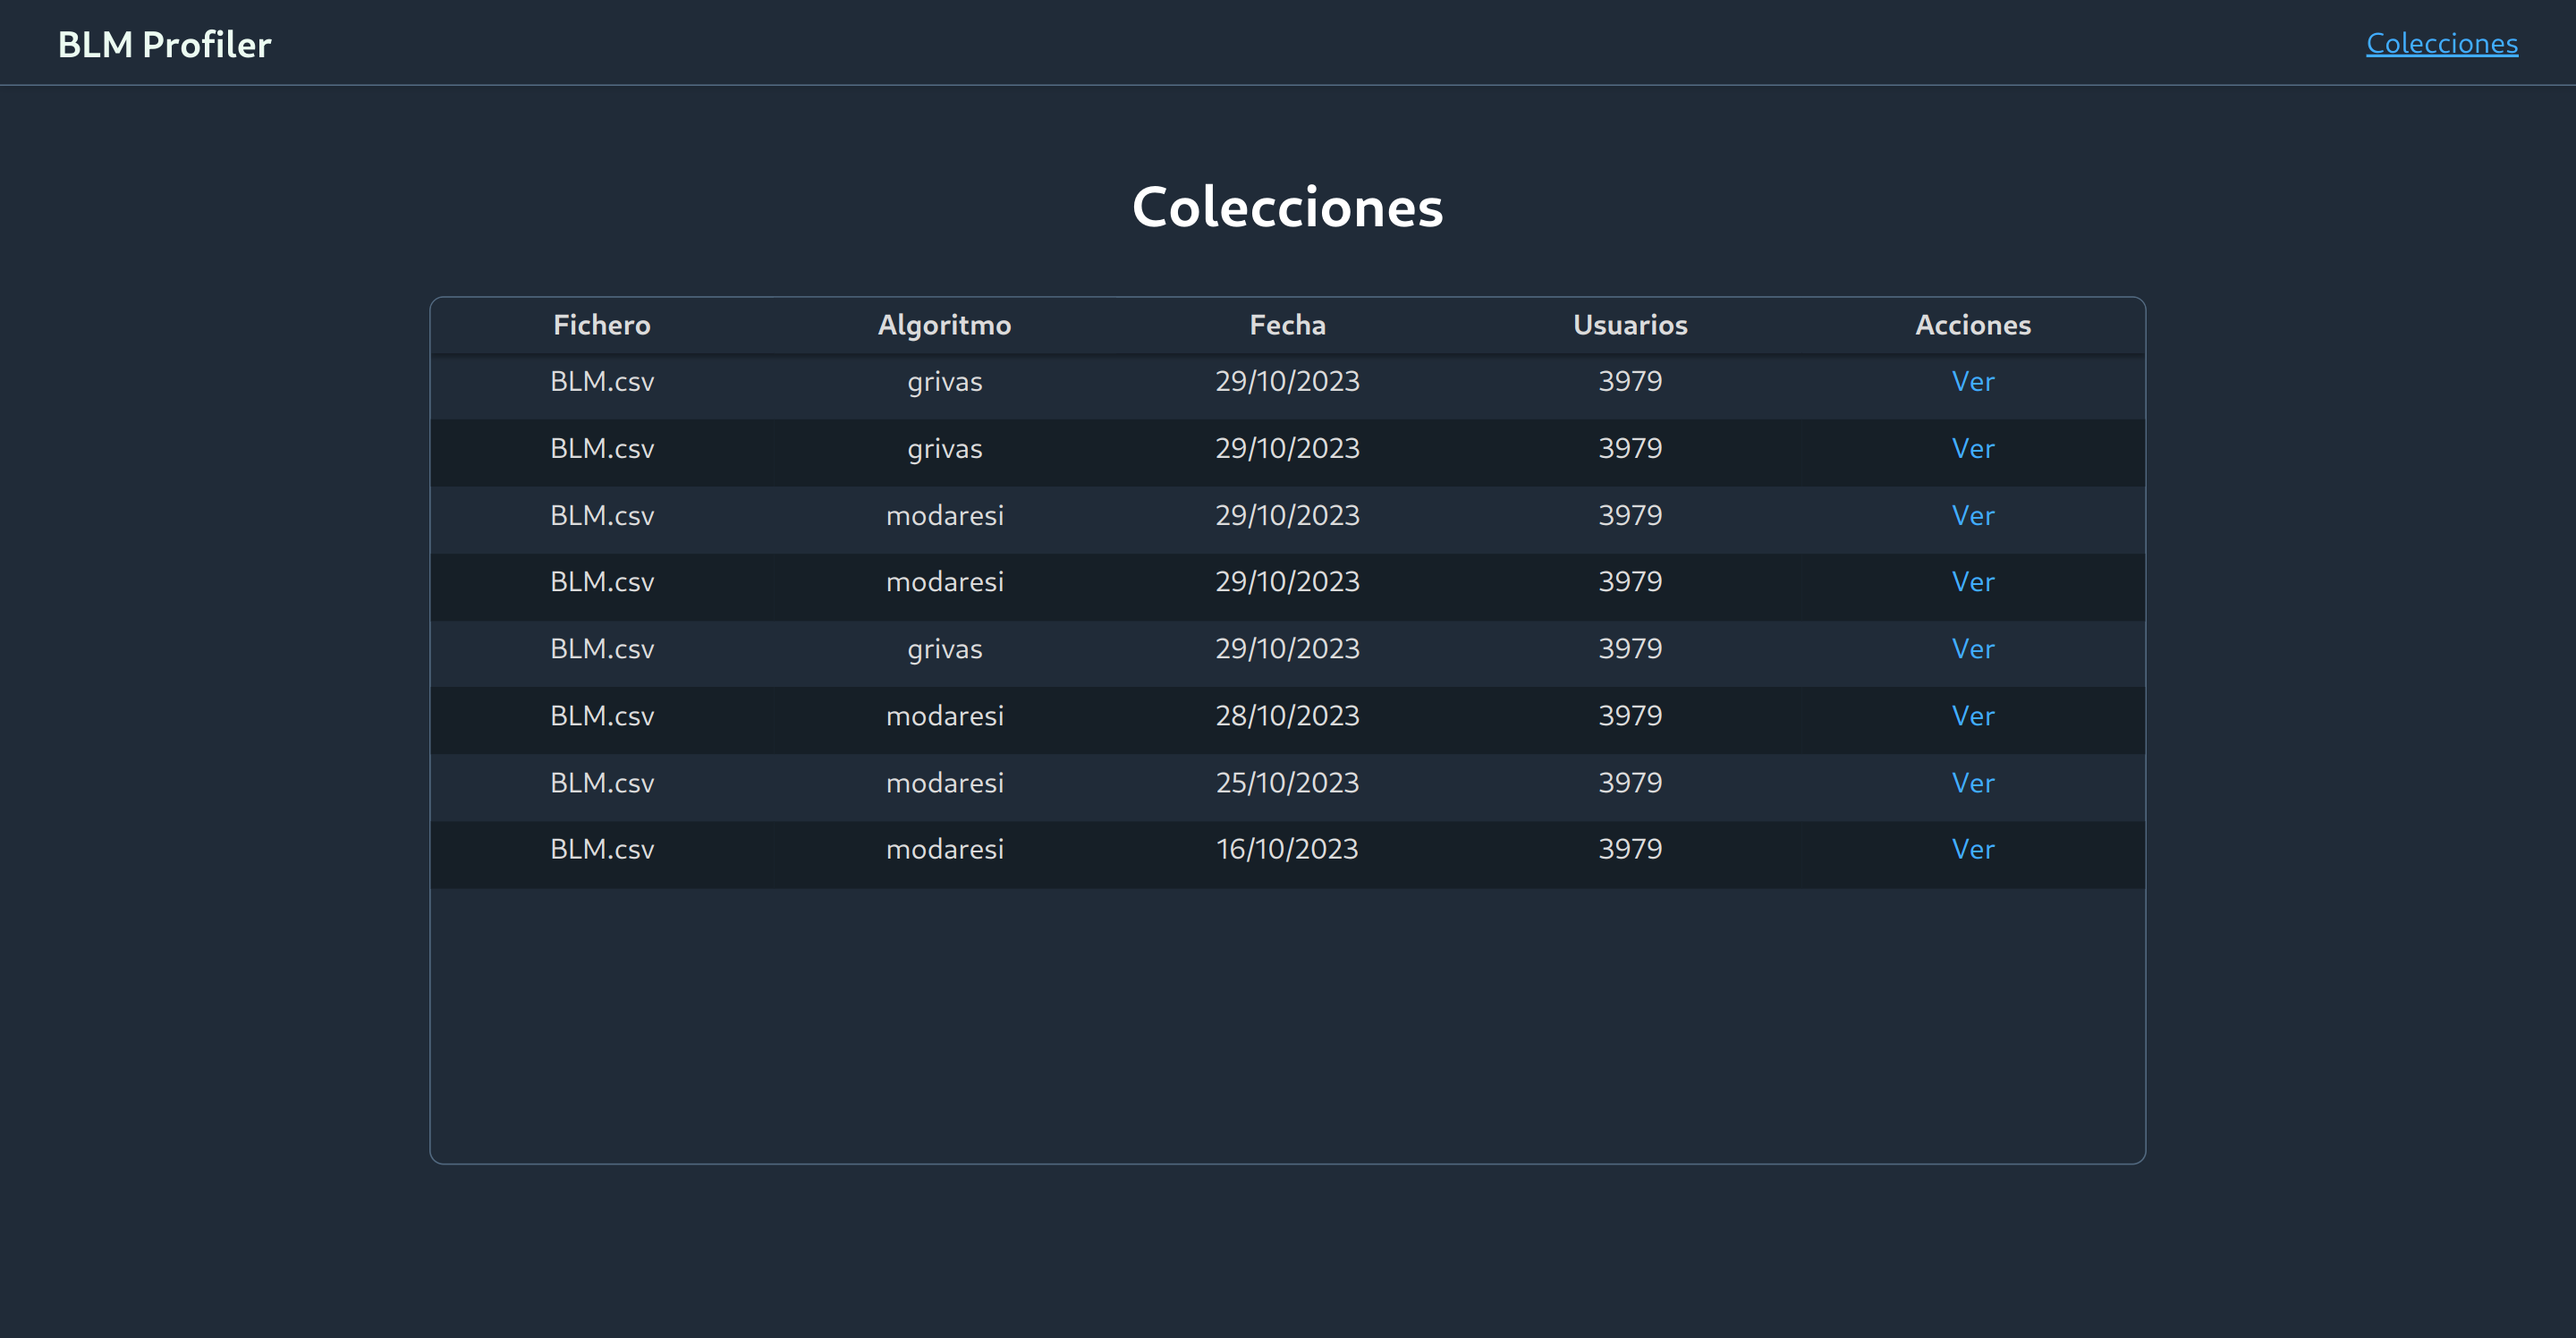
\includegraphics[width=\textwidth]{imaxes/capturas-app/desktop/colecciones.png}
  \caption{\textit{Desktop}} 
  \end{subfigure}
  \begin{subfigure}{0.2115\textwidth}
   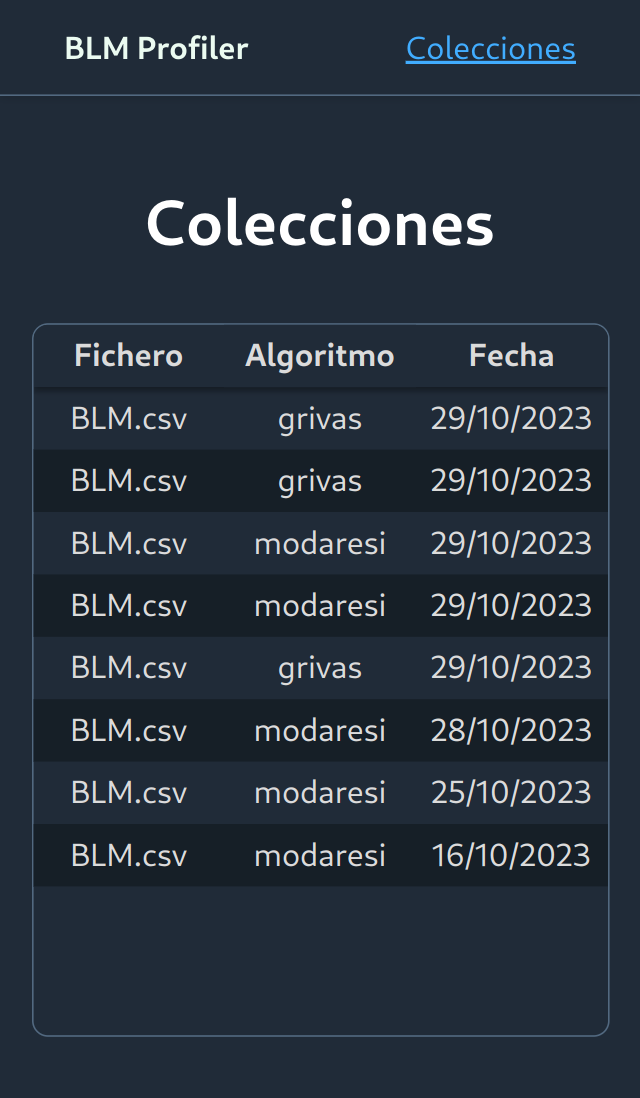
\includegraphics[width=\textwidth]{imaxes/capturas-app/mobile/colecciones.png}
  \caption{\textit{Mobile}} 
  \end{subfigure}
  \caption{Página donde se puede ver el listado de colecciones perfiladas.}
  \label{fig:app/colecciones}
\end{figure}

En esta, tendremos una tabla con las colecciones perfiladas, ordenadas cronológicamente de más a menos recientes. También podremos ver detalles como el nombre del fichero subido, la fecha de subida y el número de usuarios de la colección y algoritmo de perfilado usado en el caso de la versión \textit{desktop}. Asimismo en la columna <<Acciones>> hay un enlace llamado <<Ver>> que nos dirigirá a la página del \textit{dashboard} de esa colección. En la versión \textit{mobile} se puede navegar al \textit{dashboard} tocando sobre la fila de la colección que queramos ver.

\section{Análisis de resultados}

Tras haber explorado el funcionamiento e interfaz de la herramienta de perfilado desarrollada, se procede a una segunda fase en la que se analizan y discuten los resultados obtenidos mediante su uso.

Esta sección se dividirá en un apartado para cada algoritmo de perfilado utilizado, así como un apartado final a modo de conclusiones generales sobre los resultados de ambos \textit{profilers}.

\subsection{Algoritmo de Modaresi}
Vamos a comenzar viendo en detalle los resultados del perfilado mediante el algoritmo de modaresi (\cite{modaresi:2016}).

En cuestión de edad, se pueden observar las distribuciones de edad obtenidas  por género en la figura \ref{fig:blm/resultados-edad-moda} .Lo primero que 
llama la atención es el gran desequilibrio de usuarios en favor del grupo de 25-34 años, el cual supone prácticamente la totalidad de los mismos, un 99.8\% de la colección. Mientras que, los grupos de entre 18-24 y 35-49 solo alcanzan 9 usarios cada uno (menos del 0.1\%) y el grupo de mayores de 50 años se queda vacío. En las distribuciones de usuarios por género se mantiene en ambas la misma tendencia.

\begin{figure}[H]
  \centering
  \begin{subfigure}{0.3\textwidth}
   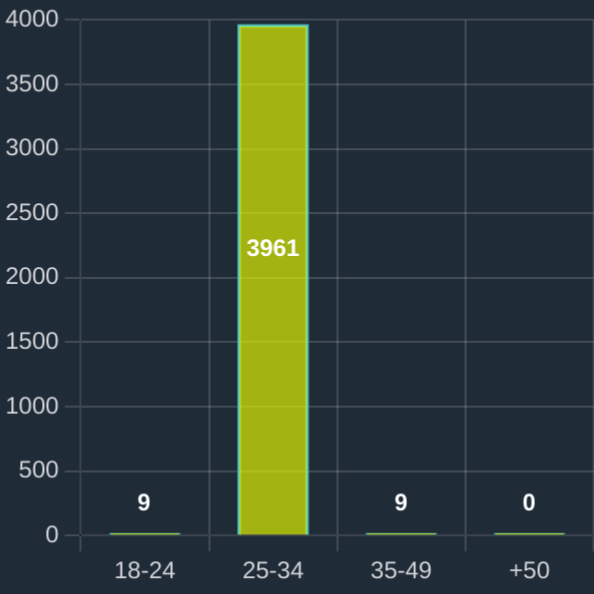
\includegraphics[width=\textwidth]{imaxes/capturas-app/graficos/modaresi/grafico-edad-moda.png}
  \caption{Edad - cualquier género}
  \label{subfig:blm/resultados-edad-moda}
  \end{subfigure}
  \begin{subfigure}{0.3\textwidth}
   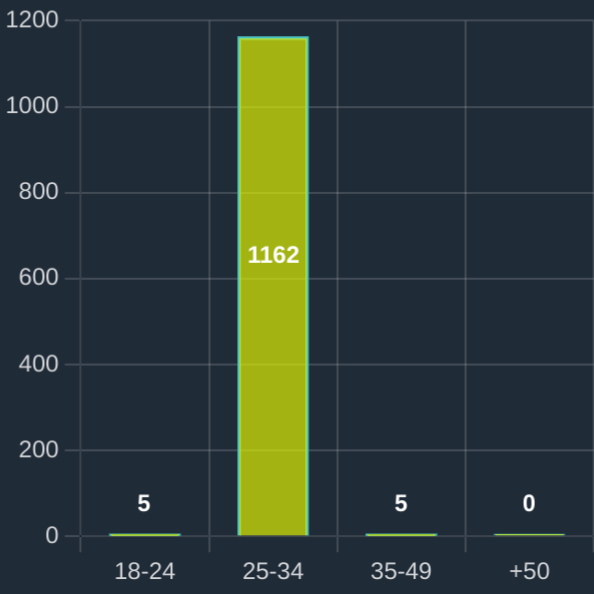
\includegraphics[width=\textwidth]{imaxes/capturas-app/graficos/modaresi/grafico-edad-moda-fem.png}
  \caption{Edad - género femenino} 
  \end{subfigure}
  \begin{subfigure}{0.3\textwidth}
   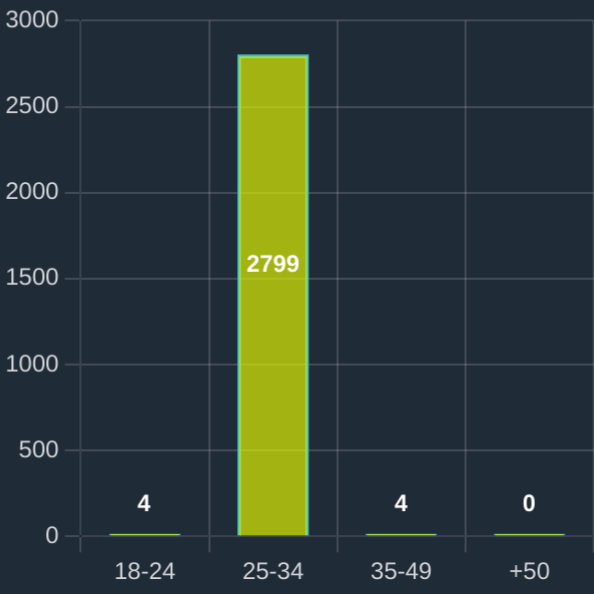
\includegraphics[width=\textwidth]{imaxes/capturas-app/graficos/modaresi/grafico-edad-moda-masc.png}
  \caption{Edad - género masculino} 
  \end{subfigure}
  \caption{Distribuciones de edad obtenidas mediante algoritmo de modaresi \cite{modaresi:2016}, en corpus \acrshort{blm} en español, según género de usuarios.}
  \label{fig:blm/resultados-edad-moda}
\end{figure}

En cuestión de género, se puede ver en el gráfico en forma de tarta de la figura \ref{fig:blm/resultados-genero-moda} que los usuarios masculinos que publicaban en \acrshort{blm} constituyen casi tres cuartas partes del total de la colección (70.72\%). Sin embargo, si vemos los gráficos por edades podemos darnos cuenta que este desequilibrio solo se da en el rango de edad de entre 25 y 34 años, ya que en el de 18-24 y 35-49 los usuarios femeninos representan más de la mitad en esos grupos demográficos. No obstante, al haber un desequilibro tan grande en cuestión de edad estas mayorías no son apenas significativas comparadas con el total de usuarios.
\begin{figure}[H]
  \centering
  \begin{subfigure}{0.3\textwidth}
   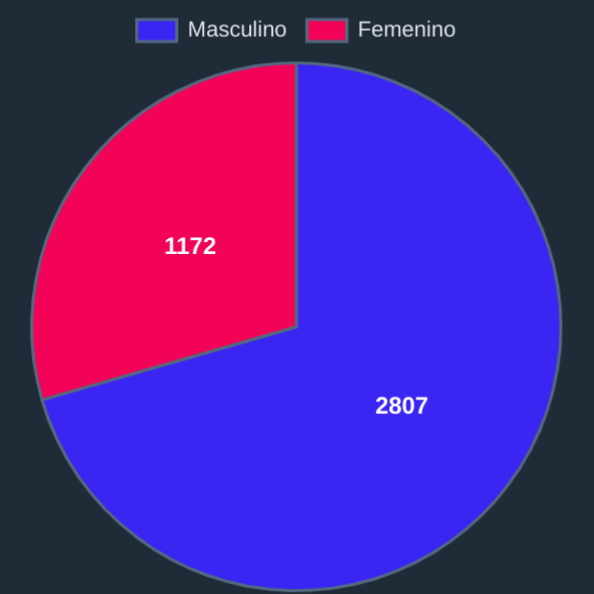
\includegraphics[width=\textwidth]{imaxes/capturas-app/graficos/modaresi/grafico-genero.png}
  \caption{Género - cualquier edad}
  \label{subfig:blm/resultados-genero-moda}
  \end{subfigure}
  \begin{subfigure}{0.3\textwidth}
   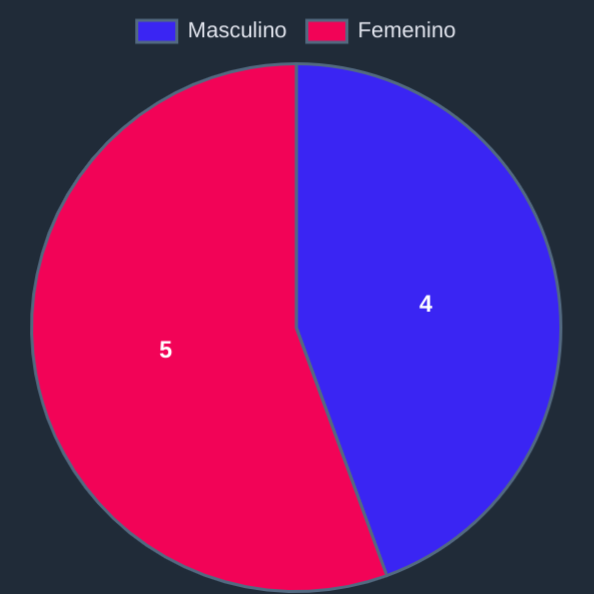
\includegraphics[width=\textwidth]{imaxes/capturas-app/graficos/modaresi/grafico-genero-jj.png}
  \caption{Género - 18-24 años}
  \end{subfigure}
  \begin{subfigure}{0.3\textwidth}
   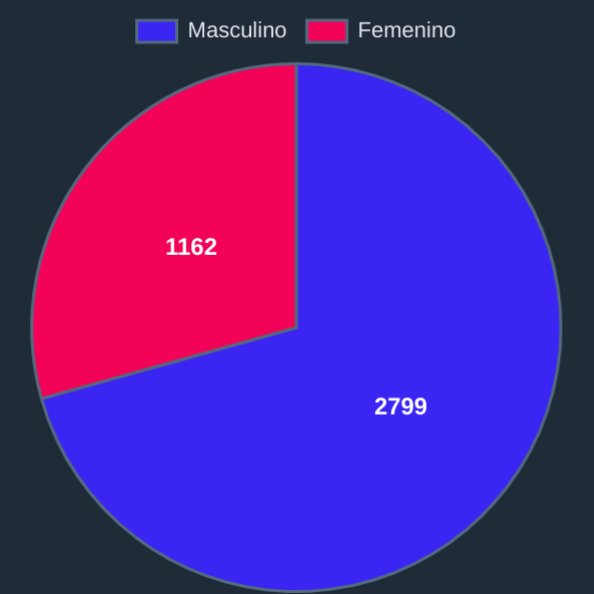
\includegraphics[width=\textwidth]{imaxes/capturas-app/graficos/modaresi/grafico-genero-j.png}
  \caption{Género - 25-34 años}
  \end{subfigure}
  \begin{subfigure}{0.3\textwidth}
   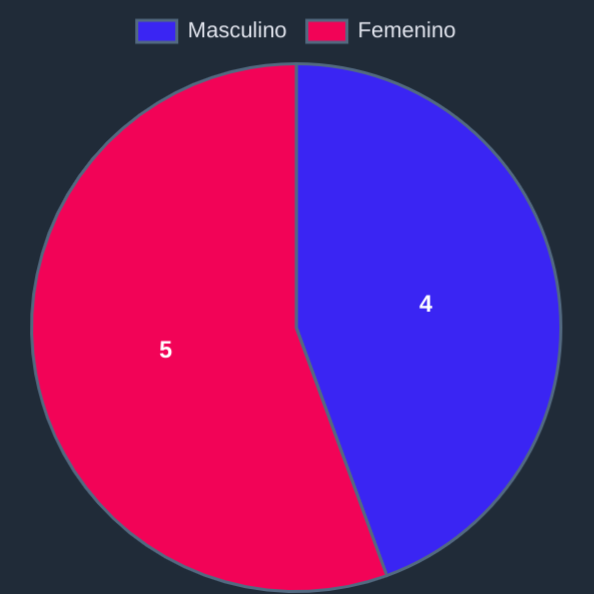
\includegraphics[width=\textwidth]{imaxes/capturas-app/graficos/modaresi/grafico-genero-v.png}
  \caption{Género - 35-49 años}
  \end{subfigure}
  \begin{subfigure}{0.3\textwidth}
   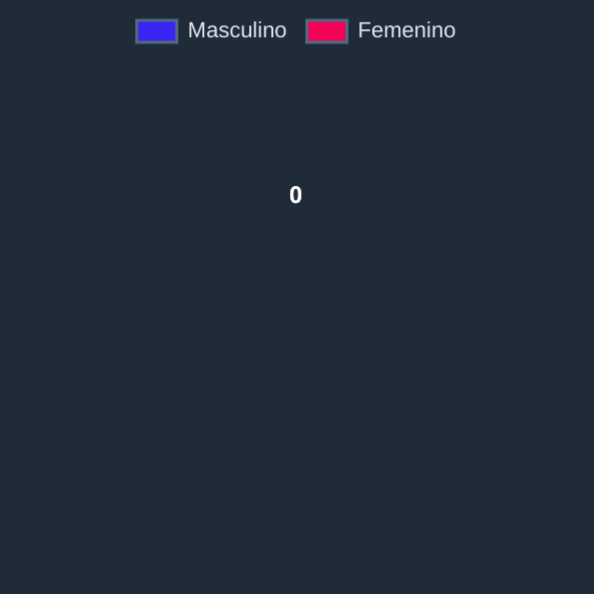
\includegraphics[width=\textwidth]{imaxes/capturas-app/graficos/modaresi/grafico-genero-vv.png}
  \caption{Género - +50 años}
  \end{subfigure}
  \caption{Distribuciones de género obtenidas mediante algoritmo de modaresi \cite{modaresi:2016}, sobre corpus \acrshort{blm} en español, según rango de edad de usuarios.}
  \label{fig:blm/resultados-genero-moda}
\end{figure}

En la tabla 
\begin{table}[H]
    \centering
    \rowcolors{2}{white}{udcgray!25}
    {
    \setlength{\tabcolsep}{0.6\tabcolsep}
    \begin{tabular}{|c|c|c|c|c|c|}
        \hline
        \rowcolor{udcpink!25}
        \diagbox{\textbf{Género}}{\textbf{Edad}} & \textbf{18-24} & \textbf{25-34} & \textbf{35-49} & \textbf{+50} & \textbf{Total} \\ \hline
        \textbf{Femenino} & 31 & 154 & 0 & 1 & 186 \\ \hline
        \textbf{Masculino} & 61 & 3725 & 3 & 4 & 3793 \\ \hline
        \textbf{Total} & 92 & 3879 & 3 & 5 & 3979 \\ \hline

    \end{tabular}%
    }
    \caption{Tabla resumen de los usuarios de la colección \acrshort{blm}.}
    \label{tab:blm/results-moda}
\end{table}

\subsection{Algoritmo de Grivas}
(\cite{grivas2015author}).

\begin{figure}[H]
  \centering
  \begin{subfigure}{0.3\textwidth}
   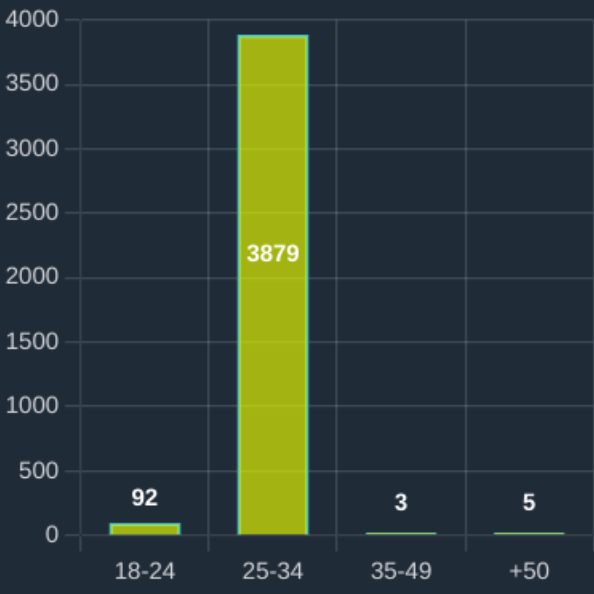
\includegraphics[width=\textwidth]{imaxes/capturas-app/graficos/grivas/grafico-edad-grivas.png}
  \caption{Edad sin filtrar} 
  \end{subfigure}
  \begin{subfigure}{0.3\textwidth}
   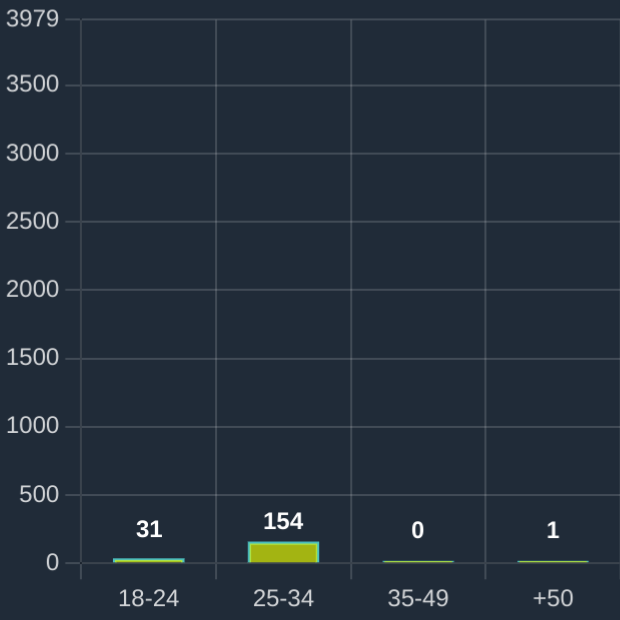
\includegraphics[width=\textwidth]{imaxes/capturas-app/graficos/grivas/grafico-edad-grivas-femenino2.png}
  \caption{Edad género femenino} 
  \end{subfigure}
  \begin{subfigure}{0.3\textwidth}
   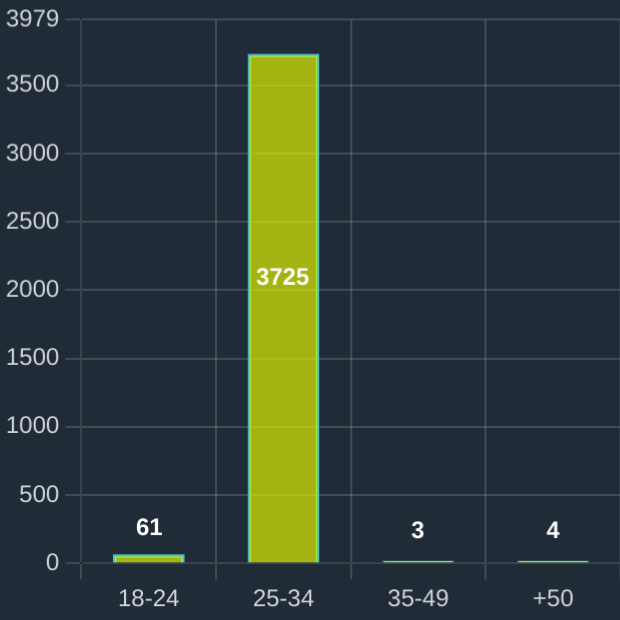
\includegraphics[width=\textwidth]{imaxes/capturas-app/graficos/grivas/grafico-edad-grivas-masculino2.png}
  \caption{Edad género masculino} 
  \end{subfigure}
  \caption{Página donde se puede ver el listado de colecciones perfiladas.}
  \label{fig:app/colecciones}
\end{figure}
\begin{figure}[H]
  \centering
  \begin{subfigure}{0.3\textwidth}
   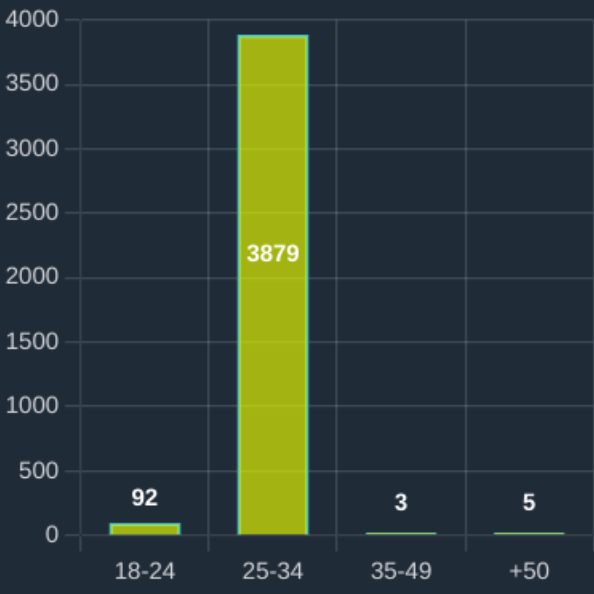
\includegraphics[width=\textwidth]{imaxes/capturas-app/graficos/grivas/grafico-edad-grivas.png}
  \caption{Edad sin filtrar} 
  \end{subfigure}
  \begin{subfigure}{0.3\textwidth}
   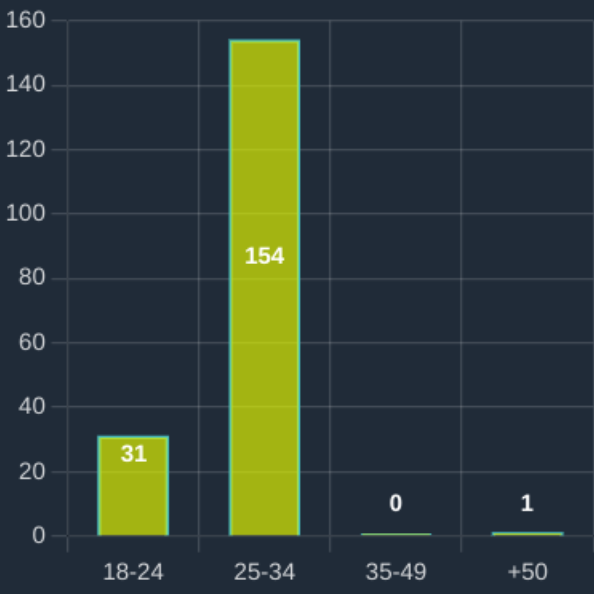
\includegraphics[width=\textwidth]{imaxes/capturas-app/graficos/grivas/grafico-edad-grivas-femenino.png}
  \caption{Edad género femenino} 
  \end{subfigure}
  \begin{subfigure}{0.3\textwidth}
   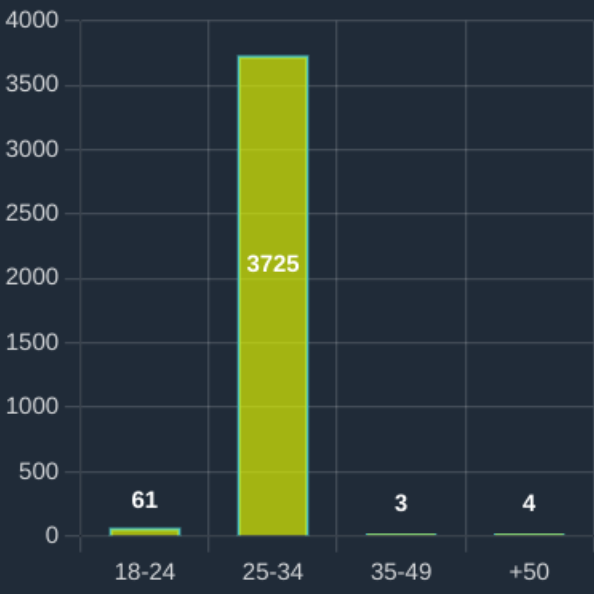
\includegraphics[width=\textwidth]{imaxes/capturas-app/graficos/grivas/grafico-edad-grivas-masculino.png}
  \caption{Edad género masculino} 
  \end{subfigure}
  \caption{Página donde se puede ver el listado de colecciones perfiladas.}
  \label{fig:app/colecciones}
\end{figure}

\begin{table}[H]
    \centering
    \rowcolors{2}{white}{udcgray!25}
    {
    \setlength{\tabcolsep}{0.6\tabcolsep}
    \begin{tabular}{|c|c|c|c|c|c|}
        \hline
        \rowcolor{udcpink!25}
        \diagbox{Género}{Edad} & 18-24 & 25-34 & 35-49 & +50 & Total \\ \hline
        Femenino & 5 & 1162 & 5 & 0 & 1172 \\ \hline
        Masculino & 4 & 2799 & 4 & 0 & 2807 \\ \hline
        Total & 9 & 3961 & 9 & 0 & 3979 \\ \hline

    \end{tabular}%
    }
    \caption{Tabla resumen de los usuarios de la colección \acrshort{blm}.}
    \label{tab:blm/results-moda}
\end{table}

\subsubsection{Edad}
\subsubsection{Género}